\documentclass[a4paper]{book}
\usepackage[nottoc,numbib]{tocbibind}
\usepackage[english]{babel}
\usepackage[pdftex]{graphics} %enable pdfgraphics support necessary for pdflatex
\usepackage{graphicx}
\usepackage{tikz}
\usepackage[small,bf]{caption}
\usepackage{footmisc}
\usepackage{sidecap}
\usepackage{fancyvrb}
\usepackage{color}
\usepackage{rotating}
\makeatletter
\setlength{\@fptop}{0pt}
\setlength{\@fpsep}{5pt}
\makeatother
\renewcommand{\dotfill}{\leaders\hbox to 5pt{\hss.\hss}\hfill}
\usepackage[hmargin=1.2cm,vmargin=1.5cm]{geometry} %set custom margins
\usepackage{fancyhdr} %enable hyperlinking, highlight page numbers
\usepackage{amsmath}
\usepackage{amssymb}
\numberwithin{equation}{subsection}
\usepackage{amsfonts}
\usepackage{mathrsfs}
\usepackage{tabularx}
\usepackage{lastpage}
\usepackage{subfigure}
\usepackage{multicol}
\usepackage{lipsum}
\usepackage{xspace}
\usepackage{latexsym} 
\usepackage{verbatim}
\usepackage{listings}
\usepackage{color}
\usepackage[usenames,dvipsnames]{xcolor}
\definecolor{listinggray}{gray}{0.9}
\definecolor{lbcolor}{rgb}{0.9,0.9,0.9}
\usepackage{listings}
\usepackage{color}

\definecolor{mygreen}{rgb}{0,0.6,0}
\definecolor{mygray}{rgb}{0.5,0.5,0.5}
\definecolor{mymauve}{rgb}{0.58,0,0.82}

\lstset{ %
   backgroundcolor=\color{white},   % choose the background color; you must add \usepackage{color} or \usepackage{xcolor}
   basicstyle=\footnotesize,        % the size of the fonts that are used for the code
   breakatwhitespace=false,         % sets if automatic breaks should only happen at whitespace
   breaklines=true,                 % sets automatic line breaking
%   captionpos=b,                    % sets the caption-position to bottom
   commentstyle=\color{mygreen},    % comment style
   deletekeywords={...},            % if you want to delete keywords from the given language
   escapeinside={\%*}{*)},          % if you want to add LaTeX within your code
   extendedchars=true,              % lets you use non-ASCII characters; for 8-bits encodings only, does not work with UTF-8
   frame=single,                    % adds a frame around the code
   keepspaces=true,                 % keeps spaces in text, useful for keeping indentation of code (possibly needs columns=flexible)
   keywordstyle=\color{blue},       % keyword style
   language=C,                 % the language of the code
   morekeywords={*,...},            % if you want to add more keywords to the set
   numbers=left,                    % where to put the line-numbers; possible values are (none, left, right)
   numbersep=5pt,                   % how far the line-numbers are from the code
   numberstyle=\tiny\color{mygray}, % the style that is used for the line-numbers
   rulecolor=\color{black},         % if not set, the frame-color may be changed on line-breaks within not-black text (e.g. comments (green here))
   showspaces=false,                % show spaces everywhere adding particular underscores; it overrides 'showstringspaces'
   showstringspaces=false,          % underline spaces within strings only
   showtabs=false,                  % show tabs within strings adding particular underscores
   stepnumber=1,                    % the step between two line-numbers. If it's 1, each line will be numbered
   stringstyle=\color{mymauve},     % string literal style
   tabsize=2,                       % sets default tabsize to 2 spaces
%   title=\lstname                   % show the filename of files included with \lstinputlisting; also try caption instead of title
% in the end language and linenumbres will be called for each block, otherwise html conversion doesn't pick up on the proper markup ...
}
% tweak the the style a little bit
\lstdefinestyle{customc}{
%   belowcaptionskip=1\baselineskip,
   breaklines=true,
   frame=single,
   xleftmargin=\parindent,
   language=C,
%   showstringspaces=false,
   basicstyle=\footnotesize\ttfamily,
   keywordstyle=\bfseries\color{green!40!black},
   commentstyle=\itshape\color{mygray},
   identifierstyle=\color{blue},
   stringstyle=\color{orange},
   framexleftmargin=5mm,
}

\lstset{escapechar=@,style=customc}
\usepackage[sort&compress,numbers]{natbib}

\pagestyle{fancy} %enable custom headeres
\fancyhead{}
\fancyfoot{} %clear predefined headers, then create your own:
\lhead{\footnotesize AliROOT Flow Package manual and documentation}
\rhead{\footnotesize The FLOW team}
\rfoot{\footnotesize Page \thepage\ of \pageref{LastPage}}
\lfoot{\footnotesize \rightmark}
\usepackage[bookmarks=true,
            bookmarksopen=true, 
            bookmarksnumbered=true, pdftex,
            hyperindex=true,linktocpage]{hyperref}
\hypersetup{
    bookmarks=true,         % show bookmarks bar?
    unicode=false,          % non-Latin characters in Acrobat’s bookmarks
    pdftoolbar=true,        % show Acrobat’s toolbar?
    pdfmenubar=true,        % show Acrobat’s menu?
    pdffitwindow=false,     % window fit to page when opened
    pdfstartview={FitH},    % fits the width of the page to the window
    pdftitle={AliROOT Flow Package manual and documentation},    % title
    pdfauthor={Redmer Alexander Bertens},     % author
    pdfsubject={AliROOT Flow Package manual and documentation},   % subject of the document
    pdfcreator={Redmer Alexander Bertens},   % creator of the document
    pdfproducer={Redmer Alexander Bertens}, % producer of the document
    pdfkeywords={ALICE} {AliROOT} {ROOT} {manual} {flow} {package} {software}, % list of keywords
    pdfnewwindow=true,      % links in new window
    colorlinks=true,       % false: boxed links; true: colored links
    linkcolor=blue,          % color of internal links
    citecolor=green,        % color of links to bibliography
    filecolor=blue,      % color of file links
    urlcolor=blue           % color of external links
}
\usepackage{lineno}
\usepackage{makeidx}
\makeindex

\sloppy
\fancypagestyle{plain}
 {
 \fancyhead{}
 \fancyfoot{}
 } % clear header and footer of plain page because of ToC

 % tikxstyle for integration of tikz graphics
 % for if in the future i'll find time for making a flowchart ...
\tikzstyle{every node}=[font=\tiny]
\tikzstyle{decision} = [rectangle, draw, fill=yellow!20, 
    rounded corners, minimum height=1.5em, minimum width=2.5em, inner sep=3pt]
\tikzstyle{decision2} = [rectangle, draw, fill=red!20, 
    rounded corners, minimum height=1.5em, minimum width=2.5em, inner sep=3pt]
\tikzstyle{decision3} = [rectangle, draw, fill=green!20, 
    rounded corners, minimum height=1.5em, minimum width=2.5em, inner sep=3pt]
\tikzstyle{block} = [rectangle, draw, fill=blue!20, 
    rounded corners, minimum height=1.5em, minimum width=2.5em, inner sep=3pt]
\tikzstyle{line} = [draw, -latex']
\tikzstyle{cloud} = [draw, ellipse,fill=red!20, 
    minimum height=2em]
\tikzstyle{sdecision} = [rectangle, draw, fill=yellow!20, 
    rounded corners, minimum height=1.5em, minimum width=2.5em, inner sep=3pt]
\tikzstyle{sblock} = [rectangle, draw, fill=blue!20, 
    rounded corners, minimum height=1.5em, minimum width=2.5em, inner sep=3pt]
\tikzstyle{scloud} = [draw, ellipse,fill=red!20, 
    minimum height=2em]
\tikzstyle{ycloud} = [draw, ellipse,fill=yellow!20, 
    minimum height=2em]

\renewcommand{\thefootnote}{\fnsymbol{footnote}}
\frontmatter

\linenumbers
\begin{document}

\noindent
\begin{center}
	\vspace*{1.5cm}
	{\LARGE \bf The FLOW Analysis Package}\\
		
	\vspace{1.5cm}
	\begin{figure}[hbt]
		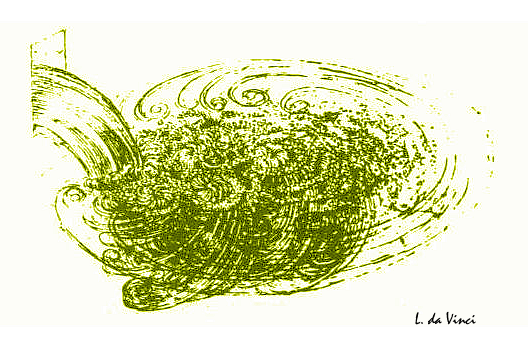
\includegraphics[width=1.\textwidth]{figs/daVinci.png}
	\end{figure}
		
	\vspace{1.5cm}
	\noindent
	{\large \bf a short manual}\\
	\today\\
\vfill
\noindent
Redmer Alexander Bertens \\ (\texttt{rbertens @ cern.ch}) \\
with excerpts from other manuals, authors of those are mentioned in text
\end{center}

\clearpage
\thispagestyle{empty}
\pagenumbering{roman}
\tableofcontents
\renewcommand{\thefootnote}{\alph{footnote}}
\mainmatter
\chapter{Introduction}
The \texttt{ALICE flow package}\index{flow package}\index{ALICE flow package|see{flow package}}\footnote{The \texttt{ALICE} flow package is part of \texttt{AliROOT}\index{AliROOT}, the ALICE extension of the \texttt{ROOT} framework, which can be obtained from \href{http://git.cern.ch/pub/AliRoot}{http://git.cern.ch/pub/AliRoot}. The flow package itself is located in the folder \texttt{\$ALICE\_ROOT/PWG/FLOW/}, where \texttt{\$ALICE\_ROOT} refers to the source directory of \texttt{AliROOT}.} contains most known flow analysis methods. The package itself consists of two parts
\begin{enumerate}
    \item The `tasks' library, which can be considered to be the \texttt{ALICE} interface to the package and takes care of e.g. track cuts, event cuts, etc;
    \item The `base' library, which is the core of the package and contains the actual implementtaion of flow analysis methods such as the scalar product method, Q-cumulant method, etc. This part of the package has no dependencies other than \texttt{ROOT} and can be used on any type of input data.
\end{enumerate}
\section{This manual}
This manual is designed to get you started with using the flow package. It is written in the following way:
\begin{itemize}
    \item Chapter \ref{sec:onthefly} is designed to get you started on a short Monte Carlo example. In this example you will use the flow package to generate toy Monte Carlo events and analyze them;
    \item Chapter \ref{sec:program} describes the flow package itself in detail. This includes a brief discussion on the structure of the package, sections on track and event cuts, an explanation of some relevant code sections and ending with an example analysis of $v_2(p_t)$ of charged pions with the Q-cumulant method. Most of this chapter pertains to the `tasks (the \texttt{AliROOT})' part of the flow package (i.e. event cuts, track cuts, PID, etc);
    \item Chapter \ref{sec:methods} gives an overview of the available flow analysis methods. For the theory behind the methods references to papers are given. Settings relevant to the specific implementation are given as well. 
    \item Lastly, chapter \ref{sec:exotic} explains how the flow package can be put to use in more `exotic' environments, such as an invariant mass method estimate of flow of rapidly decaying particles. 
    \end{itemize}
\section{Disclaimer}
What this manual is \emph{not} designed for is letting the analyzer use the flow package as a `black box'. It is supposed to be a starting point, to give an overview of the design of the software and point you to relevant classes, but in the end, the analyzer is responsible for understanding what is happening and using the software in a proper way. Configurations of the package which may work on a technical level (i.e. produce output) do not necessarily mean that the output is what you expect it to be! Always make sure that you understand what you are doing, and when in doubt, browse through the source code or consult an expert. The package is not a static entity, users are encouraged to make additions, be it track cuts, bug fixes, additional analysis methods, etc, etc. If you have suggestions, questions, commit requests, send an email to the flow-pag mailing list or to \texttt{rbertens @ cern}. 
\chapter{A Quick Start}\label{sec:onthefly}
We'll begin with a hands-on exercise in which you'll get acquainted with some aspects of the flow package in a few minutes. We'll do this by generating a few simple toy Monte Carlo events and performing a flow analysis on these simulated events without writing them (the events) to disk, a so called `flow analysis on-the-fly'\footnote{In this example the \texttt{AliFlowEventSimple} class will be used to generate toy events (which is described in detail in section \ref{sec:program}). Another on-the-fly routine is available in the \texttt{AliFlowEventSimpleMakerOnTheFly}, the original on-the-fly manual for that class is reprinted in the appendix (see \ref{sec:ante}) of this document.}. 
\section{On the fly - getting started on a Toy MC}
The steps which will be followed in this example will be the same as the steps we take when performing an analysis on data\footnote{In data, some of these steps are actually taken care of by an analysis task, but this will be described in more detail in the next chapter.}: 
\begin{enumerate}
\item Prepare your \texttt{(Ali)ROOT} session by loaded the necessary libraries
\item Create the analysis method objects
\item Initialize the methods (which creates their histograms)
\item Define track cuts
\item Create flow events, which is a container class holding all necessary information (e.g. tracks) for the flow analysis of an event (collision) and actually do the analysis
\item Finish the analysis, which will calculate the final $v_n$ values
\item Write the results to an output file
\end{enumerate}
In this Monte Carlo exercise, the flow event class will not receive data from a detector, but instead generate toy events itself. 

We will now go through these step one-by-one. All the code that is used can also be foud in the macro \texttt{runFlowOnTheFlyExample.C}\index{On the fly}\index{runFlowOnTheFlyExample.C}\footnote{In aliroot, this macro can be found at \\ \texttt{\$ALICE\_ROOT/PWGCF/FLOW/Documentation/examples/manual/runFlowOnTheFlyExample}}.
\begin{enumerate}
	\item To use the flow code the flow library needs to be loaded. In\index{libraries, AliROOT} \texttt{AliROOT}:
	\begin{lstlisting}[language=C, numbers=left]
gSystem->Load("libPWGflowBase");\end{lstlisting}
	In \texttt{root} additional libraries need to be loaded\index{libraries, ROOT}: 
        \begin{lstlisting}[language=C, numbers=left]
gSystem->Load("libGeom");
gSystem->Load("libVMC");
gSystem->Load("libXMLIO");
gSystem->Load("libPhysics");
gSystem->Load("libPWGflowBase");\end{lstlisting}
	\item We need to instantiate the flow analysis methods which we want to use. In this example we will
            instantiate two methods: one which calculates the flow versus the Monte Carlo event plane (this our reference value: as the event plane orientation is known by this method, the $v_2$ value we retrieve should be equal to the input $v_2$ by definition) and as a second method the so called Q-cumulant analysis.
\begin{lstlisting}[language=C, numbers=left]
AliFlowAnalysisWithMCEventPlane *mcep = new AliFlowAnalysisWithMCEventPlane();
AliFlowAnalysisWithQCumulants *qc = new AliFlowAnalysisWithQCumulants();\end{lstlisting}
	\item Each of the methods needs to be initialized\index{initialize methods} (e.g. to define the histograms): 
\begin{lstlisting}[language=C, numbers=left]
mcep->Init(); 
qc->Init();\end{lstlisting}
	\item To define the particles we are going to use as Reference Particles\index{reference particles} \index{RP|see{reference particles}} (RP's, particles 
	used for the {\bf Q} vector) and the Particles Of Interest\index{particles of interest} \index{POI|see{particles of interest}} (POI's, the particles of which we calculate the differential flow) we have to define two track cut objects\index{track cut object, simple}:
	\begin{lstlisting}[language=C, numbers=left]
AliFlowTrackSimpleCuts *cutsRP = new AliFlowTrackSimpleCuts();
AliFlowTrackSimpleCuts *cutsPOI = new AliFlowTrackSimpleCuts();
cutsPOI->SetPtMin(0.2);
cutsPOI->SetPtMax(2.0);	\end{lstlisting}
Particles will be selected as either POI or RP depending on whether or not they pass these cuts.
        \item Now we are ready to start the analysis. For a quick start we create a toy Monte Carlo event, tag the reference particles and particles of interest (which means that, if a particle passes the POI or RP cuts, it is flagged as `POI' or `RP')  and pass it to the two flow methods. 
	
	Since we want to analyze more than one event, this step is performed in loop. First define the number of events that need to be created, their multiplicity, and a value $v_2$ value, which can either be supplied as a fixed number (no $p_t$ dependence) of a function (to generate $p_t$ differential flow\footnote{The on the fly event generator is not limited to the generation of the second harmonic $v_2$, but to get started, this is a nice example.}
	
	\begin{lstlisting}[language=C, numbers=left]
Int_t nEvents = 1000;	// generate 1000 events
Int_t mult = 2000;		// use track multiplicity of 2000
Double_t v2 = .05;		// 5 pct integrated flow
// or sample differential flow
TF1* diffv2 = new TF1("diffv2", "((x<1.)*(0.1/1.)*x+(x>=1.)*0.1)", 0., 20.); \end{lstlisting}
	
Now we have all the ingredients to our first flow analysis	
	
	\begin{lstlisting}[language=C, numbers=left]
for(Int_t i=0; i<nEvents; i++) { 
    // make an event with mult particles 
    AliFlowEventSimple* flowevent = AliFlowEventSimple(mult,AliFlowEventSimple::kGenerate);
    // modify the tracks adding the flow value v2
    flowevent->AddV2(diffv2);
    // select the particles for the reference flow
    flowevent->TagRP(cutsRP);
    // select the particles for differential flow
    flowevent->TagPOI(cutsPOI);
    // do flow analysis with various methods:
    mcep->Make(flowevent);
    qc->Make(flowevent);
    // delete the event from memory
    delete flowevent;
} \end{lstlisting}
	\item To fill the histograms which contain the final results we have to call Finish for each method:
	\begin{lstlisting}[language=C, numbers=left]
mcep->Finish(); 
qc->Finish(); \end{lstlisting}
	\item This concludes the analysis and now we can write the results into a file. Two options for writing the input to a file are available: 
     \begin{itemize}
     \item Create a new output file and write the output to this file
     \begin{lstlisting}[language=C, numbers=left]
TFile *outputFile = new TFile("outputMCEPanalysis.root","RECREATE");
mcep->WriteHistograms();
TFile *outputFile = new TFile("outputQCanalysis.root","RECREATE");
qc->WriteHistograms();\end{lstlisting}

Please note that this will create a new output file, and overwrite any existing filse called \texttt{AnalysisResults.root}.

\item  To write the output of multiple analyses into subdirectories of one file, one can do the following:
\begin{lstlisting}[language=C, numbers=left]
TFile *outputFile = new TFile("AnalysisResults.root","RECREATE");
TDirectoryFile* dirQC = new TDiretoryFile("outputQCanalysis", "outputQCanalysis");
qc->WriteHistograms(dirQC);
TDirectoryFile* dirMCEP = new TDiretoryFile("outputMCEPanalysis", "outputMCEPanalysis");
mcep->WriteHistograms(dirMCEP);
\end{lstlisting}
\end{itemize}

Note that \texttt{AnalysisResults.root} \index{AnalysisResults.root} is the default name given to analyses in \texttt{AliROOT}. Many macros in \texttt{AliROOT} will expect a file \texttt{AnalyisResults.root} as input, so for most users it will be convenient to follow this convention.

When done with running the analysis, do not forget to write the file to disk by calling
\begin{lstlisting}[language=C, numbers=left]
TFile::Close();	// write the buffered file to disk \end{lstlisting}
\end{enumerate}

\section{What is in the output file ?}
\index{output file} Now we have written the results into a file, but what is in there? 

Although the output of different flow analysis techniques might differ slightly as a result of their different approaches at estimating $v_2$, the output files containers are always constructed in a similar way. 

\subsection{AliFlowCommonHists - Output objects}\label{sec:commonhists}
Objects of two types are stored in the output of the flow analysis\footnote{Make sure that \texttt{libPWGflowBase.so} is loaded in your \texttt{(Ali)ROOT} session, otherwise these objects will be unknown.}
\begin{enumerate}
\item \texttt{AliFlowCommonHist}\index{AliFlowCommonHist}, which is a class that contains common histograms for the flow analysis (e.g. QA histograms and histograms that contain the analysis flags which were used). Depending on the type of flow analysis that was used, this object contains histograms from the following list:
\begin{lstlisting}[language=C, numbers=left]
  Bool_t    fBookOnlyBasic;       // book and fill only control histos needed for all methods
  TH1F*     fHistMultRP;          // multiplicity for RP selection
  TH1F*     fHistMultPOI;         // multiplicity for POI selection
  TH2F*     fHistMultPOIvsRP;     // multiplicity for POI versus RP
  TH1F*     fHistPtRP;            // pt distribution for RP selection
  TH1F*     fHistPtPOI;           // pt distribution for POI selection
  TH1F*     fHistPtSub0;          // pt distribution for subevent 0
  TH1F*     fHistPtSub1;          // pt distribution for subevent 1
  TH1F*     fHistPhiRP;           // phi distribution for RP selection
  TH1F*     fHistPhiPOI;          // phi distribution for POI selection
  TH1F*     fHistPhiSub0;         // phi distribution for subevent 0
  TH1F*     fHistPhiSub1;         // phi distribution for subevent 1
  TH1F*     fHistEtaRP;           // eta distribution for RP selection
  TH1F*     fHistEtaPOI;          // eta distribution for POI selection
  TH1F*     fHistEtaSub0;         // eta distribution for subevent 0
  TH1F*     fHistEtaSub1;         // eta distribution for subevent 1
  TH2F*     fHistPhiEtaRP;        // eta vs phi for RP selection
  TH2F*     fHistPhiEtaPOI;       // eta vs phi for POI selection
  TProfile* fHistProMeanPtperBin; // mean pt for each pt bin (for POI selection)
  TH2F*     fHistWeightvsPhi;     // particle weight vs particle phi
  TH1F*     fHistQ;               // Qvector distribution
  TH1F*     fHistAngleQ;          // distribution of angle of Q vector
  TH1F*     fHistAngleQSub0;      // distribution of angle of subevent 0 Q vector
  TH1F*     fHistAngleQSub1;      // distribution of angle of subevent 1 Q vector
  TProfile* fHarmonic;            // harmonic 
  TProfile* fRefMultVsNoOfRPs;    // <reference multiplicity> versus # of RPs
  TH1F*     fHistRefMult;         // reference multiplicity distribution
  TH2F*     fHistMassPOI;         // mass distribution for POI selection \end{lstlisting}
  This information is from the header file of the AliFlowCommonHist object\footnote{The headers of both output objects can be found in \texttt{\$ALICE\_ROOT/PWG/FLOW/Base/}.}
  \item \texttt{AliFlowCommonHistResults}\index{AliFlowCommonHistResults} is an object designed to hold the common results of the flow analysis\footnote{The word common here is used to indicate histograms that hold observables which are evaluated in all flow analysis methods. Specific analysis methods may however store additional histograms which are not covered in this list!}. The possible common histograms stored in this object are
  \begin{lstlisting}[language=C, numbers=left]
  TH1D* fHistIntFlow; // reference flow
  TH1D* fHistChi;     // resolution
  // RP = Reference Particles:  
  TH1D* fHistIntFlowRP;     // integrated flow of RPs
  TH1D* fHistDiffFlowPtRP;  // differential flow (Pt) of RPs
  TH1D* fHistDiffFlowEtaRP; // differential flow (Eta) of RPs
  // POI = Particles Of Interest:
  TH1D* fHistIntFlowPOI;     // integrated flow of POIs
  TH1D* fHistDiffFlowPtPOI;  // differential flow (Pt) of POIs
  TH1D* fHistDiffFlowEtaPOI; // differential flow (Eta) of POIs \end{lstlisting}
  
  \end{enumerate}
  The titles of the histograms in the output object differ from the names of the pointers given in the two lists printed above, but the lists give an overview of what is available; the easiest way however of getting acquainted with where to find histograms in the output is browsing them in \texttt{ROOT's TBrowser}\index{TBrowser} (see figure \ref{fig:browserExample}).
  \begin{lstlisting}[language=C, numbers=left]
  new TBrowser(); \end{lstlisting}
\begin{SCfigure}
 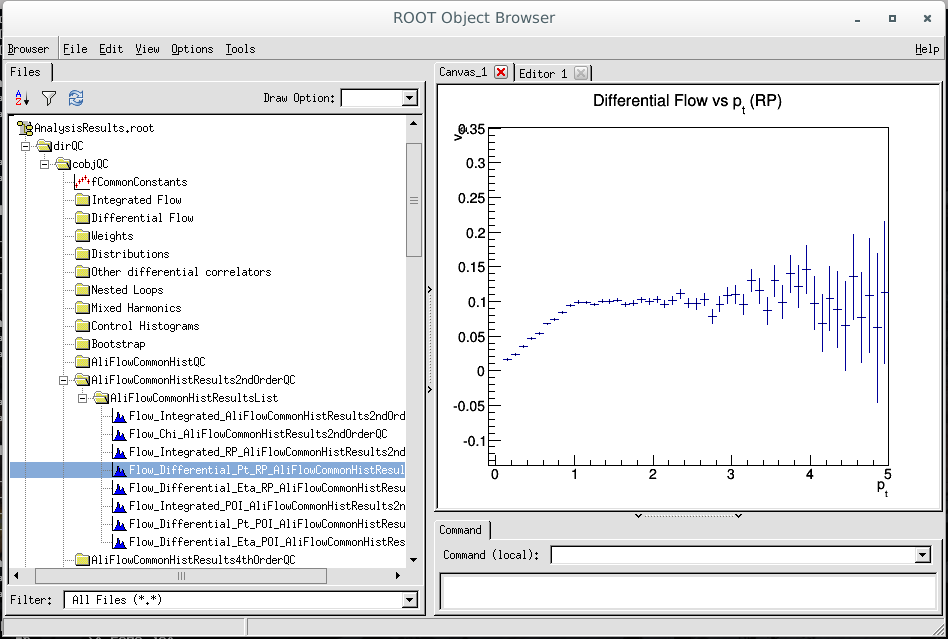
\includegraphics[width=0.70\textwidth]{figs/browserExample.png}
 \caption[TBrowser with output file]{Example of output file opened in a TBrowser, results of differential $v_2$ analysis with second order Q-cumulant analysis are shown.}
 \label{fig:browserExample}
\end{SCfigure}

The \texttt{AliFlowCommonHist} and \texttt{AliFlowCommonHistResults} classes are derived from the generic \texttt{TNamed}\index{TNamed} \texttt{ROOT} object and can be written to a \texttt{ROOT} file. The flow analysis tasks will, as output, write the complete \texttt{AliFlowCommonHist} and \texttt{AliFlowCommonHistResults} objects to file at the end of an analysis. To read the content of these objects, the \texttt{libPWGflowBase} library must be loaded in your \texttt{ROOT} session. 

\subsubsection{Comparing flow results}
A convenient way of comparing the results of the different flow analysis strategies that have been used is invoking the macro \texttt{compareFlowResults.C}\footnote{\texttt{\$ALICE\_ROOT/PWGCF/FLOW/macros/compareFlowResults.C}}\index{compareFlowResults}.  This macro will read the analysis output file \texttt{AnalysisResults.root}, extract the requested results from it and plot them. For a full overview of what can be done with the macro, the reader is referred to the macro itself and its ample documentation. To run the macro on the dataset that we have just generated, simply do
\begin{lstlisting}[language=C, numbers=left]
.L compareFlowResults.C
compareFlowResults(TSring(""))	// the empty suffix indicates on the fly events \end{lstlisting}

\begin{SCfigure}
 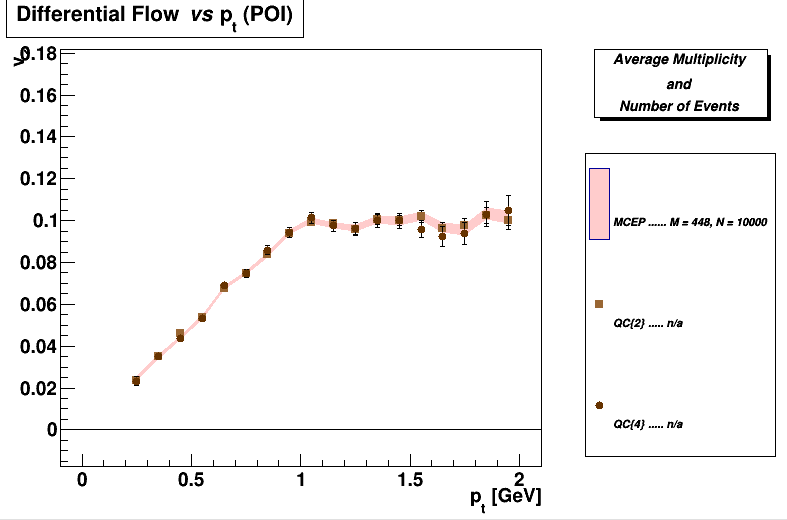
\includegraphics[width=0.70\textwidth]{figs/compareFlowResults.png}
 \caption[Comparing on the fly flow results]{Example of inspecting the output file of the on the fly analysis with the \texttt{compareFlowResults.C macro}.}
 \label{fig:browserExample}
\end{SCfigure}


\chapter{The Program}\label{sec:program}
The basic idea behind the flow package is that from whatever input you have, a \emph{flow event}\index{flow event} is constructed, which is then passed to one or more flow analysis methods\index{flow analysis method} (e.g. the scalar product method\index{scalar product} or Q-cumulant\index{Q-cumulant} method). The flow event is a collection of \emph{flow tracks}\index{flow track}, which are simple objects carrying only the kinematic information that is necessary to do flow analysis. By setting up the flow package in this way, the flow analysis methods can analyze input from various sources, be it ALICE data, Monte Carlo events, STAR data, etc, etc, as long as the flow event is properly filled\index{STAR input} \index{Monte Carlo input}. This might all sound a bit abstract at this point; this chapter however will explain all details and relevant classes in detail. For those who are impatient and prefer seeing the flow package in action, section \ref{sec:example} gives a step-by-step example of doing a $\pi^{\pm}$ $v_2$ analysis in the \texttt{AliROOT} analysis framework. 

\section{Overview}
\begin{figure}
\begin{center}
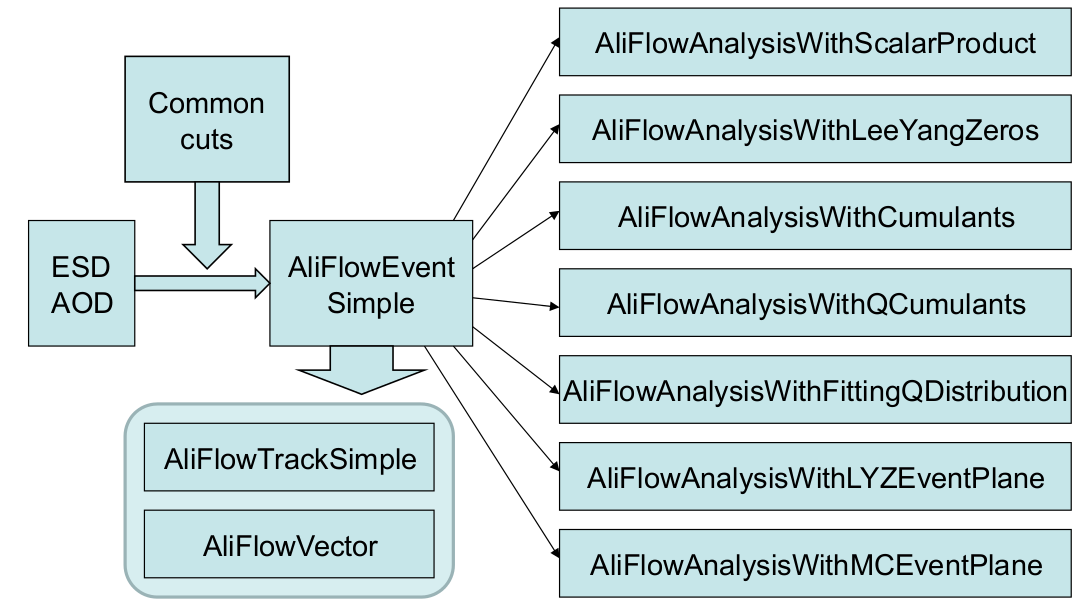
\includegraphics[width=.75\textwidth]{figs/flowChart.png}
\caption{Schematic presentation of the organization of the flow package. Input, which can come from any kind of source, is converted to a generic \texttt{AliFlowEventSimple} object, which in turn is passed to the analysis methods.}
\label{fig:flowchart}
\end{center}
\end{figure}
Figure \ref{fig:flowchart} gives a simple schematic representation\index{flowchart} of the flow package. Input events (in the case of the figure this is either ESDs or AODs) pass a set of event cuts (the common cuts) and are then converted to a flow event (stored as an \texttt{AliFlowEventSimple}\index{AliFlowEventSimple} object). This flow event holds a collection of flow tracks (\texttt{AliFlowTrackSimple}\index{AliFlowTrackSimple} objects) which are passed to flow analysis methods. The only steps of this flow chart which depend on \texttt{AliROOT} libraries are the ones handling \texttt{ALICE} data types (the ESDs or AODs). The rest of the analysis chain (the \texttt{AliFlowEventSimle} and the analysis methods) have no specific \texttt{AliROOT} dependence and are just simple \texttt{c++} objects. Therefore, the flow package is split into two libraries
\begin{description}
    \item [libPWGflowBase] \index{libPWGflowBase}The base library, which has no specific \texttt{AliROOT} dependencies. This library holds objects such as the \texttt{AliFlowEventSimple} and \texttt{AliFlowTrackSimple}, and analysis methods classes. The analysis methods classes follow the naming scheme: \texttt{AliFlowAnalysisWith$\ast$} where $\ast$ denotes a specific analysis method. All classes which end up in the \text{libPWGflowBase.so} shared object can be found in \texttt{\$ALICE\_ROOT/PWG/FLOW/Base};
    \item [libPWGflowTasks] \index{libPWGflowTasks} The tasks library, which has specific \texttt{AliROOT} dependencies. Contrary to what the name suggests, this library does not just hold tasks, but actually comprises all classes of the flow package which need to include \texttt{AliROOT} specific classes. This ranges from classes to read the AOD or ESD input data (important examples are the \texttt{AliFlowEvent}\index{AliFlowEvent} and \texttt{AliFlowTrackCuts}\index{AliFlowTrackCuts}, which will be discussed later on in this chapter) and the \texttt{AliAnalysisTask$\ast$} classes, which are analysis tasks, derived from \texttt{AliAnalysisTaskSE} which can be used in the \texttt{AliROOT} analysis framework and are actually just interface classes to the underlying flow analysis methods of libPWGflowBase. The classes which are bundled into the \text{libPWGflowTasks.so} shared object can be found in \texttt{\$ALICE\_ROOT/PWG/FLOW/Tasks};
\end{description}
Some tools, such as the flow event or track cuts, have a `base' component which name ends with the suffix `simple', and an `tasks' (\texttt{AliROOT}) component which does not have this suffix. The `tasks' class in these cases inherits from the `base' class. 

\section{Flow Event}\index{flow event}
Every flow analysis in the flow package starts with the flow event. As mentioned earlier, the flow event is a simple container class which holds a collection of flow tracks, which are in turn fed to the flow analysis methods. 
\subsection{Input data}\index{input data}
Before passing the flow event to the flow analysis methods, it needs to be filled with a set of flow tracks. In general, a distinction is made between \emph{reference particles} (or \emph{RP's}), which are particles that are used to build the \textbf{Q} vector(s), and \emph{particles of interest} (or \emph{POI's}), which are the particles of which you'll calculate the differential flow. The flow event and the flow analysis methods are designed to keep track of which flow tracks are POI's, RP's (or even both at the same time), which is important to avoid auto-correlation effects which can distort the $v_n$ measurement. The user of the flow package however is responsible for properly setting up the analysis! 

The flow event can be filled with input from many sources. In the second chapter of this manual, a simple method has been shown where the flow event (the \texttt{AliFlowEventSimple} object) fills itself by generating a set of Monte Carlo tracks by sampling kinematic variables from supplied p.d.f.'s. Using this method is a very effective tool for testing and developing new flow analysis methods (if you generate events with a certain $v_2(p_t)$ and then retrieve the same $v_2(p_t)$ from your flow analysis method, you can use that as a tool to proof the validation of your analysis method) but if you want to do a data analysis, a somewhat more advanced - but not difficult - approach is necessary. 

Filling a flow event from data can be performed either `by-hand' (which is covered in section \ref{sec:exotic} on more exotic analyses), but the most commonly used method of filling a flow event in the \texttt{AliROOT} analysis framework is using the dedicated task \texttt{AliAnalysisTaskFlowEvent}\index{AliAnalysisTaskFlowEvent}. 

The idea behind this is the following:
\begin{enumerate}
\item Setup the \texttt{AliAnalysisTaskFlowEvent} task to receive input events (e.g. \texttt{AODs}, \texttt{ESDs}, \texttt{MC}, $\ldots$;
\item Define two sets of track selection criteria (colloquially referred to as \emph{track cuts}), one for POI's and one for RP's;
\item Pass these two sets of track cuts to the \texttt{AliAnalysisTaskFlowEvent};
\item The \texttt{AliAnalysisTaskFlowEvent} will convert the tracks  of each input event to a set of \texttt{AliFlowSimpleTracks}. Depending on whether or not a track passes the track selection for POI's or RP's, the \texttt{AliFlowSimpleTrack} is labeled as a POI or RP (or both. In the case where a track does not meet any of the track selection criteria, it is omitted from the \texttt{AliFlowSimpleTrack} collection and not added to the flow event);
\item All the \texttt{AliFlowSimpleTracks} are added to the flow event which is passed to the flow analysis methods. 
\end{enumerate}

\subsection{Event selection}\index{event selection}
When using the \texttt{AliAnalysisTaskFlowEvent} task to create your flow event, the \texttt{AliAnalysisTaskFlowEvent} task is responsible for ensuring that only good quality tracks enter into your analysis by making sensible track selections. The first step however at safeguarding track quality is making sure that the events that are accepted by \texttt{AliAnalysisTaskFlowEvent} pass sane event selection criteria. 

\subsubsection{Trigger selection}\index{event selection!trigger selection}
A certain combination a of detector signals (a \emph{trigger}) is required for an event to be written to storage. Different types of analyses might require different types of events, and hence, different types of triggers. 

You can set a trigger by calling
\begin{lstlisting}[language=C, numbers=left]
AliAnalysisTaskFlowEvent::SelectCollisionCandidates(UInt_t offlineTriggerMask);\end{lstlisting}
where \texttt{offlineTriggerMask} is the trigger mask corresponding to the desired trigger. A list of all available triggers, with a short descrption, can be found in the header file of the \texttt{AliVEvent} class\footnote{\texttt{\$ALICE\_ROOT/...}}. This function, however, is not implement in the \texttt{AliAnalysisTaskFlowEvent} itself, but rather in the base class of which most of the analysis task classes within \texttt{AliROOT} are derived: the \texttt{AliAnalysisTaskSE} class (which is designed to handle a single event, hence the suffix `SE'). For each event that is written from a file, but function \texttt{AliAnalysisTaskSE::Exec()} is called, which - among other things - checks if an event passes the requested trigger selection, and if so, calls the \texttt{UserExec()} function of your analysis task. In the case of the \texttt{AliAnalysisTaskFlowEvent} this is the \texttt{AliAnalysisTaskFlowEvent::UserExec()}, which creates \texttt{AliFlowSimpleTracks} and fills the flow event. 

A general remark about trigger selection in flow analyses is that the non-uniform acceptance correction methods that are implemented in the flow package assume a flat \textbf{Q} vector distribution. Specific triggers (e.g. EMCal triggers) result in a \textbf{Q} vector bias which should \emph{not} be corrected as they invalidate that assumption. A safe approach is therefore using a minimum bias trigger for your analysis (such as \texttt{AliVEvent::kMB}), other triggers selections will not a-priori lead to problems, but use them with caution!

\subsubsection{Event cuts}\index{event selection!event cuts}
In addition to trigger selection, generally one wants to perform additional event (quality) selection. The flow package contains an event cuts class which can be used to perform event selection, the \texttt{AliFlowEventCuts} object\footnote{\texttt{\$ALICE\_ROOT/PWG/FLOW/Tasks/AliFlowEventCuts.cxx}}. \index{AliFlowEventCuts}

To use the event cuts object in combination with the \texttt{AliAnalysisTaskFlowEvent} task, simply create the event cuts object, configure it and pass it to the \texttt{AliAnalysisTaskFlowEvent}:
\begin{lstlisting}[language=C, numbers=left]
  AliFlowEventCuts* cutsEvent = new AliFlowEventCuts("EventCuts");
  // configure some event cuts, e.g. centrality
  cutsEvent->SetCentralityPercentileRange(20., 30.);
  // pass it to the flow event task via the setter
  AliAnalysisTaskFlowEvent::SetCutsEvent(cutsEvent);\end{lstlisting}

  The available cut parameters in the flow event cuts object are\index{event selection!parameters}
\begin{lstlisting}[language=C, numbers=left]
  Bool_t fCutNumberOfTracks;//cut on # of tracks
  Int_t fNumberOfTracksMax;  //limits
  Int_t fNumberOfTracksMin;  //limits
  Bool_t fCutRefMult; //cut on refmult
  refMultMethod fRefMultMethod; //how do we calculate refmult?
  Bool_t fUseAliESDtrackCutsRefMult; //use AliESDtrackCuts for refmult calculation
  AliESDtrackCuts::MultEstTrackType fRefMultMethodAliESDtrackCuts;
  Int_t fRefMultMax; //max refmult
  Int_t fRefMultMin; //min refmult
  AliFlowTrackCuts* fRefMultCuts; //cuts
  AliFlowTrackCuts* fMeanPtCuts; //mean pt cuts
  AliFlowTrackCuts* fStandardTPCcuts; //Standard TPC cuts
  AliFlowTrackCuts* fStandardGlobalCuts; //StandardGlobalCuts
  Bool_t fCutPrimaryVertexX; //cut on x of prim vtx
  Double_t fPrimaryVertexXmax; //max x prim vtx
  Double_t fPrimaryVertexXmin; //min x prim vtx
  Bool_t fCutPrimaryVertexY; //cut on y of prim vtx
  Double_t fPrimaryVertexYmax; //max y prim vtx
  Double_t fPrimaryVertexYmin; //min y prim vtx
  Bool_t fCutPrimaryVertexZ; //cut on z of prim vtx
  Double_t fPrimaryVertexZmax; //max z prim vtx
  Double_t fPrimaryVertexZmin; //min z prim vtx
  Bool_t fCutNContributors; //cut on number of contributors
  Int_t fNContributorsMax; //maximal number of contrib
  Int_t fNContributorsMin; //minimal number of contrib
  Bool_t fCutMeanPt; //cut on mean pt
  Double_t fMeanPtMax; //max mean pt
  Double_t fMeanPtMin; //min mean pt
  Bool_t fCutSPDvertexerAnomaly; //cut on the spd vertexer anomaly
  Bool_t fCutSPDTRKVtxZ; //require compatibility between SPDvertexz TRKvertexz
  Bool_t fCutTPCmultiplicityOutliers; //cut TPC multiplicity outliers
  Bool_t fCutTPCmultiplicityOutliersAOD; // cut TPC outliers in 10h or 11h aod
  Bool_t fUseCentralityUnchecked; //use the unchecked method
  refMultMethod fCentralityPercentileMethod; //where to get the percentile from
  Bool_t fCutZDCtiming;   //cut on ZDC timing
  AliTriggerAnalysis fTrigAna; //trigger analysis object
  Bool_t fCutImpactParameter; //cut on impact parameter (MC header)
  Double_t fImpactParameterMin; // min impact parameter
  Double_t fImpactParameterMax; // max impact parameter
  TH2F *fhistTPCvsGlobalMult; //!correlation between TPCMult and GlobalMult
  Bool_t fData2011; //2011 data is used\end{lstlisting}
  all of which are accessible via dedicated setters\index{event selection!setters},
\begin{lstlisting}[language=C, numbers=left]
  void SetNumberOfTracksMax(Int_t value) {fNumberOfTracksMax=value;fCutNumberOfTracks=kTRUE;}
  void SetNumberOfTracksMin(Int_t value) {fNumberOfTracksMin=value;fCutNumberOfTracks=kTRUE;}
  void SetNumberOfTracksRange(Int_t min, Int_t max) {fNumberOfTracksMin=min;fNumberOfTracksMax=max;fCutNumberOfTracks=kTRUE;}
  void SetRefMultMax(Int_t value) {fRefMultMax=value;fCutRefMult=kTRUE;}
  void SetRefMultMin(Int_t value) {fRefMultMin=value;fCutRefMult=kTRUE;}
  void SetRefMultRange(Int_t min, Int_t max) {fRefMultMin=min;fRefMultMax=max;fCutRefMult=kTRUE;}
  void SetImpactParameterMax(Double_t value) {fImpactParameterMax=value;fCutImpactParameter=kTRUE;}
  void SetImpactParameterMin(Double_t value) {fImpactParameterMin=value;fCutImpactParameter=kTRUE;}
  void SetImpactParameterRange(Double_t min, Double_t max) {fImpactParameterMin=min;fImpactParameterMax=max;fCutImpactParameter=kTRUE;}
  void SetPrimaryVertexXrange(Double_t min, Double_t max)
  void SetPrimaryVertexYrange(Double_t min, Double_t max)
  void SetPrimaryVertexZrange(Double_t min, Double_t max)
  void SetNContributorsRange(Int_t min, Int_t max=INT_MAX) 
  void SetMeanPtRange(Double_t min, Double_t max) {fCutMeanPt=kTRUE; fMeanPtMax=max; fMeanPtMin=min;}
  void SetCutSPDvertexerAnomaly(Bool_t b=kTRUE) {fCutSPDvertexerAnomaly=b;}
  void SetCutZDCtiming(Bool_t c=kTRUE) {fCutZDCtiming=c;}
  void SetCutSPDTRKVtxZ(Bool_t b=kTRUE) {fCutSPDTRKVtxZ=b;}
  void SetCutTPCmultiplicityOutliers(Bool_t b=kTRUE) {fCutTPCmultiplicityOutliers=b;}  
  void SetCutTPCmultiplicityOutliersAOD(Bool_t b=kTRUE) {fCutTPCmultiplicityOutliersAOD=b;}
  void SetRefMultMethod(refMultMethod m) {fRefMultMethod=m;}
  void SetRefMultMethod(AliESDtrackCuts::MultEstTrackType m) { fRefMultMethodAliESDtrackCuts=m; 
  void SetRefMultCuts( AliFlowTrackCuts* cuts ) {fRefMultCuts=static_cast<AliFlowTrackCuts*>(cuts->Clone());}
  void SetMeanPtCuts( AliFlowTrackCuts* cuts ) {fMeanPtCuts=static_cast<AliFlowTrackCuts*>(cuts->Clone());}
  void SetQA(Bool_t b=kTRUE) {if (b) DefineHistograms();}
  void SetCentralityPercentileMethod( refMultMethod m) {fCentralityPercentileMethod=m;}
  void SetUseCentralityUnchecked(Bool_t b=kTRUE) {fUseCentralityUnchecked=b;}
  void SetUsedDataset(Bool_t b=kTRUE) {fData2011=b;}    // confusing name, better use different interface
  void SetLHC10h(Bool_t b=kTRUE) {fData2011=(!b);}      // TODO let cut object determine runnumber and period
  void SetLHC11h(Bool_t b=kTRUE) {fData2011=b;}         // use this only as 'manual override'\end{lstlisting}

\subsubsection{Caveats and remarks}  
Some caveats\index{event selection!caveats} and remarks about using the event cuts object
\begin{description}
\item[Default behavior] By default, the event cuts object accepts all events. All desired cuts have to be set by the user. This is also reflected in the design of the setters: most of the setters will, when called, set a \texttt{Bool\_t} to true which enables a cut on a certain parameter;
\item[Applicability of cuts to different datatypes] \index{event selection!data types}Not all the cuts can be applied to all input data types. In e.g. the process of filtering \texttt{AODs} from \texttt{ESDs}, `technical' event cuts are made and not all events are stored in the \texttt{AOD} format. Because of this, information that can be rqeuired from \texttt{ESDs} might not be available (as it is not necessary) in \texttt{AODs}. To see whether or not a cut you set is actually applied to the datatype you're using, take a look at
\begin{lstlisting}[language=C, numbers=left]
Bool_t AliFlowEventCuts::PassesCuts(AliVEvent *event, ALIMCEvent *mcevent)\end{lstlisting}
This function determines whether or not an event is accepted: it starts by converting the virtual event type that is passed as argument to either an \texttt{ESD} or \texttt{AOD} event, and goes through selection criteria accordingly. 
\item[Event cuts outside of the \texttt{AliAnalysisTaskFlowEvent} class]
When you perform a flow analysis without using the \texttt{AliAnalysisTaskFlowEvent} class (which is done e.g. in the analyses explained in section \ref{sec:exotic}), you can still use the event cuts class by creating an instance of the object, passing it to your analsyis class and `manually' checking the return value of the function 
\begin{lstlisting}[language=C, numbers=left]
Bool_t AliFlowEventCuts::PassesCuts(AliVEvent *event, ALIMCEvent *mcevent)\end{lstlisting}
\item[Data taking period] Most event cuts will be tuned specifically to the LHC10h or LHC11h data taking periods. The event cuts class might need to be updated to accomodate specific cuts for different periods - do not hesitate write patches for this!
\end{description}
for e.g. each event that is passed to your \texttt{::UserExec()} function.

\section{Track cuts and the track cuts object}\index{track selection}
As explained in the previous subsection, flow events are filled with tracks which fulfill certain track selection criteria. These criteria are checked using the \texttt{AliFlowTrackCuts} class. The \texttt{AliFlowTrackCuts} class can handle different types of input from diffferent data-types (e.g. \texttt{ESD} or \texttt{AOD}) and information from different sub-detector systems. All input is in the end converted to \texttt{AliFlowSimpleTracks} which are added to the flow event. To understand how the \texttt{AliFlowTrackCuts}\index{AliFlowTrackCuts} object works and how it should be configured, it is good to make a few distinctions and remarks. 

The term `track' is generally used for reconstructed particle trajectories which are constructed from information coming from the tracking detectors in central barrel of the \texttt{ALICE} detector (more specifically from information from the \texttt{ITS} and \texttt{TPC} detectors). Tracks are the most commonly used data source, and the translation from `track' to \texttt{AliFlowTrackSimple} is trivial, as it merely comprises copying  kinematic information ($p_t$, $\varphi$, $\eta$) from the barrel track to the \texttt{AliFlowTrackSimple} object. 

When using information that is not coming from tracking detectors, e.g. information from the \texttt{VZERO}\index{VZERO} system, this procedure of simply copying variables is not suitable as the \texttt{VZERO} system does not measure $p_t$, $\varphi$, $\eta$ of particles, but is an array of scintillators with limited spatial resolution. Nevertheless, the \texttt{AliFlowTrackCuts} class converts the \texttt{VZERO} signal to \texttt{AliFlowTrackSimples} which are, to the flow event, indistinguishable from barrel tracks. As the procedure of accepting these tracks is very different from the procedure of accepting barrel tracks, they will be treated separately in the following subsections. 

\subsection{ESD tracks as data source}\index{track selection!ESD tracks}
The safest and most convenient way of using \texttt{ESD} tracks as a data source is by using one of the pre-defined track cuts sets that are available in the \texttt{AliFlowTrackCuts} class. These sets of track cuts mimic the cuts that are defined in the \texttt{AliESDtrackCuts} class\footnote{\texttt{\$ALICE\_ROOT/ANALYSIS/AliESDtrackCuts.cxx}}. The following default track cuts sets are available:
\begin{lstlisting}[language=C, numbers=left]
  static AliFlowTrackCuts* GetStandardTPCStandaloneTrackCuts();
  static AliFlowTrackCuts* GetStandardTPCStandaloneTrackCuts2010();
  static AliFlowTrackCuts* GetStandardGlobalTrackCuts2010();
  static AliFlowTrackCuts* GetStandardITSTPCTrackCuts2009(Bool_t selPrimaries=kTRUE);
  static AliFlowTrackCuts* GetStandardMuonTrackCuts(Bool_t isMC=kFALSE, Int_t passN=2);
  \end{lstlisting}
All these are static methods which create a new track cuts object and configure it properly, so to use these track cuts it suffices to type e.g.
\begin{lstlisting}[language=C, numbers=left]
AliFlowTrackCuts* myCuts = AliFlowTrackCuts::GetStandardGlobalTrackCuts2010();\end{lstlisting}
To get a better understanding of what the \texttt{AliFlowTrackCuts} class actually does, let's take a look at what how the cut object is configured in this case:
\begin{lstlisting}[language=C, numbers=left]
AliFlowTrackCuts* AliFlowTrackCuts::GetStandardGlobalTrackCuts2010()
{
  //get standard cuts
  AliFlowTrackCuts* cuts = new AliFlowTrackCuts("standard Global tracks");
  cuts->SetParamType(kGlobal);
  cuts->SetPtRange(0.2,5.);
  cuts->SetEtaRange(-0.8,0.8);
  cuts->SetMinNClustersTPC(70);
  cuts->SetMinChi2PerClusterTPC(0.1);
  cuts->SetMaxChi2PerClusterTPC(4.0);
  cuts->SetMinNClustersITS(2);
  cuts->SetRequireITSRefit(kTRUE);
  cuts->SetRequireTPCRefit(kTRUE);
  cuts->SetMaxDCAToVertexXY(0.3);
  cuts->SetMaxDCAToVertexZ(0.3);
  cuts->SetAcceptKinkDaughters(kFALSE);
  cuts->SetMinimalTPCdedx(10.);
  return cuts;
}\end{lstlisting}
The configuration falls into three categories:
\begin{enumerate}
\item A number of track quality cuts is set;
\item Some kinematic cuts are set;
\item The parameter type\index{track selection!parameter type} is set by calling \texttt{AliFlowTrackCuts::SetParamType()} (in this case to \texttt{AliFlowTrackCuts::kGlobal}). This last step is of particular importance as it takes care disentangling the POI and RP selection and removing a $v_n$ bias due to auto-correlations. When the flow event is filled (the relevant piece of code is printed under section \ref{sec:fill}), a check is done to see if the POI's and RP's are of the same type. If not, a track cannot be a POI and RP at the same time (as they are from different sources). However, if POI's and RP's originate from the same source, an \texttt{AliFlowTrackSimple} can be both a POI and RP at the same time if it satisfies both the POI and RP track selection criteria. By specifying the parameter type by calling \texttt{AliFlowTrackCuts::SetParamType()} the flow event is configured to properly deal with overlapping or exclusive POI and RP selections. A wrongly configured parameter type can lead to double counting of tracks and nonsensical analysis results! The following list of track parameter types is available as an \texttt{enum} in \texttt{AliFlowTrackCuts.h}
\begin{lstlisting}[language=C, numbers=left]
  enum trackParameterType { kMC, 
                            kGlobal, 
                            kTPCstandalone, 
                            kSPDtracklet,
                            kPMD,
                            kV0,    //neutral reconstructed v0 particle
                            kVZERO, //forward VZERO detector
                            kMUON,
                            kKink,
                            kAODFilterBit,
                            kUserA,     // reserved for custom cuts
                            kUserB      // reserved for custom cuts
                          };\end{lstlisting}
Note that \texttt{kV0} is reserved to denote a decay vertex of a neutral particle, and \texttt{kVZERO} is used to indicate the VZERO detector system. kUserA and kUserB are additional flags which can selected for `custom' track selection sets.
\end{enumerate}

\subsection{AOD tracks as data source}\index{track selection!AOD tracks}
\texttt{AOD} tracks are derived from \texttt{ESD} tracks via process called `fitlering'. If an \texttt{ESD} track meets a pre-defined set of track cuts, it is converted to an \texttt{AOD} track which is stored in an \texttt{AOD} event. The \texttt{AOD} track carries a specific flag (called \texttt{filterbit}) which corresponds to the specific set of cuts that was applied to create accept the track. A full list of track selection criteria corresponding to distinct filterbits can be found \href{}{here}. Note that different \texttt{AOD} productions might have different filterbit definitions!

In \texttt{AOD} analysis it generally suffices to select tracks of a certain filterbit, instead of checking quality criteria `by-hand' as is done in \texttt{ESD} analyses (some variables which one would cut on in \texttt{ESD} tracks might not even be available in the \texttt{AOD} tracks as the \texttt{AOD} is designed to be a light-weight `end-user' data format). To get an instance of the \texttt{AliFlowTrackCuts} object which only selects tracks based on a specific filterbit\index{track selection!AOD filterbit}\index{filterbit}, one can call
\begin{lstlisting}[language=C, numbers=left]
 static AliFlowTrackCuts* GetAODTrackCutsForFilterBit(UInt_t bit = 1);\end{lstlisting}
 which is defined as
 \begin{lstlisting}[language=C, numbers=left]
 AliFlowTrackCuts* AliFlowTrackCuts::GetAODTrackCutsForFilterBit(UInt_t bit)
{
  // object which in its default form only cuts on filterbit (for AOD analysis)
  AliFlowTrackCuts* cuts = new AliFlowTrackCuts(Form("AOD fitlerbit %i", (int)bit));
  cuts->SetMinimalTPCdedx(-999999999);
  cuts->SetAODfilterBit(bit);
  cuts->SetParamType(AliFlowTrackCuts::kAODFilterBit);
  return cuts;
}  \end{lstlisting}
The \texttt{SetMinimalTPCdedx(-999999999);} is kept here for backward-compatibility. 

Note that also in the case of \text{AOD} analyses the parameter type is set to (if necessary) decouple POI and RP selections. 

\subsection{Additional options}
As stated, input data needn't necessarily come in the form of barrel tracks - we can use other detector systems as well. When dealing with barrel tracks, quality criteria might not be the only thing you want to select your tracks on: perhaps you want to do analysis on identified particles. The following sub-sections explain how the \texttt{AliFlowTrackCuts} object can be used to achieve this. 

\subsubsection{Identified particles}\index{track selection!particle identification}\index{particle identification}
The \texttt{AliFlowTrackCuts} object can do particle selection for a number of particles that are defined in the AliPID\footnote{\texttt{\$ALICE\_ROOT/STEER/STEERBas/AliPID.h}}. To enable 
particle identification as a selection criterion, call the function
\begin{lstlisting}[language=C, numbers=left]
void AliFlowTrackCuts::SetPID(
    AliPID::EParticleType pid, 
    PIDsource s=kTOFpid, 
    Double_t prob=0.9)
{fParticleID=pid; fPIDsource=s; fParticleProbability=prob; fCutPID=kTRUE; InitPIDcuts();
}\end{lstlisting}
The first argument specifies the particle species that will be selected via the \texttt{EParticleType} enum. The total list of particles as defined in the  \texttt{AliPID} class reads
\begin{lstlisting}[language=C, numbers=left]
  enum EParticleType {
    kElectron = 0, 
    kMuon = 1, 
    kPion = 2, 
    kKaon = 3, 
    kProton = 4, 

    kDeuteron = 5,
    kTriton = 6,
    kHe3 = 7,
    kAlpha = 8,
    
    kPhoton = 9,
    kPi0 = 10, 
    kNeutron = 11, 
    kKaon0 = 12, 
    kEleCon = 13,
    
    kUnknown = 14
  };\end{lstlisting}
  Note that not all these particles may be available for selection via \texttt{AliFlowTrackCuts}!
  
  The second argument tells the \texttt{AliFlowTrackCuts} class which particle identification method\index{particle identification!methods} should be used. The available methods are
  \begin{lstlisting}[language=C, numbers=left]
    enum PIDsource {
                   kTPCpid,      // default TPC pid (via GetTPCpid)
                   kTOFpid,      // default TOF pid (via GetTOFpid)
                   kTOFbayesian, // TOF bayesian pid (F.Noferini)
                   kTOFbeta,     // asymmetric cuts of TOF beta signal
                   kTPCdedx,      // asymmetric cuts of TPC dedx signal
                   kTOFbetaSimple, //simple TOF only cut
                   kTPCbayesian, //bayesian cutTPC
	           kTPCNuclei,   // added by Natasha for Nuclei
                   kTPCTOFNsigma // simple cut on combined tpc tof nsigma
                   };\end{lstlisting}
                   
The third argument (with a default value of 0.9) gives the analyzer control over the purity of the particle sample by setting a lower bound on the probability that a particle is of a certain species (where 0 would mean no selection and 1 -theoretically - means a 100\% pure sample). To see how - and if - this parameter is used in a certain identification routine, take a look at the source code.
                   
The best way of understanding how particles are identified is by just browsing the relevant pieces of the code in the \texttt{AliFlowTrackCuts.cxx} file (look at the list of \texttt{Passes$\ast$Cuts()}, but to give a very short overview:
\begin{description}
\item[kTPCpid] Return particle identity as stored in the \texttt{AliESDtrack}, TPC information only;
\item[kTOFpid] Return particle identify as stored in the \texttt{AliESDtrack}, TOF information only;
\item[kTOFbayesian] Combined TPC and TOF Bayesian PID method;
\item[kTOFbeta] PID based on asymmetric TOF $\beta$ cut;
\item[kTPCdedx] PID cut using TPC $\frac{dE}{dx}$ measurements stored in the \texttt{AliESDtrack},
\item[kTOFbetaSimple] PID cut based on TOF time stored in the \texttt{AliESDtrack};
\item[kTPCbayesian] Bayesian cut based on TPC or TOF signal;
\item[kTPCNuclei] PID selection for heavy nuclei;
\item[kTPCTOFNsigma]  Cut based in a simple combined cut on the $n$-$\sigma$ signal from TPC and TOF, requires PID response object. The PID response object is created by the PID response task, and thus requires that the PID response task runs in an analysis train \emph{before} the \texttt{AliFlowTrackCuts} class does its selection. To enable the PID response task, add the following lines to your run macro:
\begin{lstlisting}[language=C, numbers=left]
gROOT->LoadMacro("ANALYSIS/macros/AddTaskPIDResponse.C");
AddTaskPIDResponse();\end{lstlisting}
The default value for $n$-$\sigma$ is 3, but it can be set to a different 
value using
\begin{lstlisting}[language=C, numbers=left]
void AliFlowTrackCuts::SetNumberOfSigmas(Float_t val);\end{lstlisting}
\end{description}

\subsubsection{Caveats and notes}
\index{particle identification!caveats}
\begin{description}
\item[Applicability of cuts to different data types] Just as not all event and track cuts that are available for all data types. For the track quality cuts this has been explained in the previous subsections, but one has to reqlize that in addition, not all particle identification methods are available for all types of data. At the time of writing, the \texttt{ESD} particle identification is more elaborate than the \texttt{AOD} counterpart. To see which PID methods exist for the different data types, check the \texttt{AliFlowTrackCuts::Passes$\ast$pidCut()} functions,  printed below for your convenience.

\begin{lstlisting}[language=C, numbers=left]
Bool_t AliFlowTrackCuts::PassesAODpidCut(const AliAODTrack* track )
{
     if(!track->GetAODEvent()->GetTOFHeader()){
          AliAODPid *pidObj = track->GetDetPid();
          if (!pidObj) fESDpid.GetTOFResponse().SetTimeResolution(84.);
          else{
            Double_t sigmaTOFPidInAOD[10];
            pidObj->GetTOFpidResolution(sigmaTOFPidInAOD);
            if(sigmaTOFPidInAOD[0] > 84.){
              fESDpid.GetTOFResponse().SetTimeResolution(sigmaTOFPidInAOD[0]); // use the electron TOF PID sigma as time resolution (including the T0 used)
          }
        }
     }

 //check if passes the selected pid cut for ESDs
  Bool_t pass = kTRUE;
  switch (fPIDsource)
  {
   case kTOFbeta:
      if (!PassesTOFbetaCut(track)) pass=kFALSE;
      break;
  case kTOFbayesian:
      if (!PassesTOFbayesianCut(track)) pass=kFALSE;
      break;
  case kTPCbayesian:
      if (!PassesTPCbayesianCut(track)) pass=kFALSE;
      break;
  case kTPCTOFNsigma:
      if (!PassesTPCTOFNsigmaCut(track)) pass = kFALSE;
      break;
  default:
    return kTRUE;
    break;
 }
  return pass;

}
//-----------------------------------------------------------------------
Bool_t AliFlowTrackCuts::PassesESDpidCut(const AliESDtrack* track )
{
  //check if passes the selected pid cut for ESDs
  Bool_t pass = kTRUE; 
  switch (fPIDsource)    
  {
    case kTPCpid:
      if (!PassesTPCpidCut(track)) pass=kFALSE;
      break;
    case kTPCdedx:
      if (!PassesTPCdedxCut(track)) pass=kFALSE;
      break;
    case kTOFpid:
      if (!PassesTOFpidCut(track)) pass=kFALSE;
      break;
    case kTOFbeta:
      if (!PassesTOFbetaCut(track)) pass=kFALSE;
      break;
    case kTOFbetaSimple:
      if (!PassesTOFbetaSimpleCut(track)) pass=kFALSE;
      break;
    case kTPCbayesian:
      if (!PassesTPCbayesianCut(track)) pass=kFALSE;
      break;
    case kTOFbayesian:
      if (!PassesTOFbayesianCut(track)) pass=kFALSE;
      break;
    case kTPCNuclei:
      if (!PassesNucleiSelection(track)) pass=kFALSE;
      break;
    case kTPCTOFNsigma:
      if (!PassesTPCTOFNsigmaCut(track)) pass = kFALSE;
      break;
    default:
      printf("AliFlowTrackCuts::PassesCuts() this should never be called!\n");
      pass=kFALSE;
      break;
  }
  return pass;
}\end{lstlisting}
In general, particle identification is not a trivial procedure, and one needs to find a balance between purity and efficiency. Which particle identification to choose depends heavily on the desired outcome of the analysis. In case of e.g. a high-precision measurement of $\pi$ $v_2$, a method which has a very high purity but low efficiency can be chosen: $\pi$'s are an abundant particle species and high precision requires high purity. On the other hand, if one does selection for kaons to reconstruct $\varphi$-mesons, loose cuts with high efficiency can be chosen, as the $\varphi$-meson is a rare probe and invariant mass requirements on the kaon pairs will take care of mis-identifications. 

To get access to QA information on track selection \emph{before} and \emph{after} PID cuts, the QA mode of the \texttt{AliFlowTrackCuts} can be selected.

\item[Track cuts outside of the \texttt{AliAnalysisTaskFlowEvent} class] Just as the flow event cuts can be used outside of the \texttt{AliAnalysisTaskFlowEvent} class, one can use the \texttt{AliFlowTrackCuts} class in a similar way, by calling, for each track,
\begin{lstlisting}[language=C, numbers=left]
Bool_t AliFlowTrackCuts::IsSelected(TObject* obj, Int_t id)\end{lstlisting}
or directly one of the \texttt{PassesCuts($\ast$)} functions which \texttt{IsSelected()} calls. 
\end{description}

\subsubsection{VZERO}\index{track selection!VZERO}\index{VZERO}
Now that the barrel tracks have been explained, let's continue to the treatment of VZERO information. The VZERO detector consists of two scintillator arrays at opposite sides of the interaction point (VZEROA and VZEROC) each containing 32 readout channels. To convert the VZERO information to \texttt{AliFlowTrackCuts}, two steps are taken:
\begin{enumerate}
\item A `track' is built from a VZERO tile by taking the geometric mean of the tile as the track direction (from which $\eta$ and $\varphi$ can be constructed);
\item The VZERO analogue signal strength within a VZERO tile (which is proportional to charge deposition) is taken as a weight when evaluating the total \textbf{Q} vector.
\end{enumerate}
As there is no straightforward way to convert VZERO multiplicity to $p_t$, the VZERO signal can in principle not be used as POI in the flow analysis, neither can a $p_t$ range be selected when using the VZERO as RP selection. In addition to this, the `raw' VZERO signal itself cannot be used directly for flow analysis  but needs to be calibrated tile-by-tile. To understand how this calibration is performed in the flow package, we need to go into a little bit of detail on how to build a \textbf{Q} vector. 

In general, a \textbf{Q} vector is defined as
\begin{equation}\label{qvzero}
\mbox{\textbf{Q}} = \sum_{\mbox{tracks}} w_i \exp \left( i n \varphi \right)
\end{equation}
where $w_i$ is a track weight, $n$ is the harmonic, and $\varphi$ is the azimuthal angle of a track.  As explained, in the case of VZERO tiles, $\varphi$ is derived from the position of the VZERO tile and $w_i$ is the VZERO signal which is proportional to multiplicity. However, not all VZERO tiles are equally sensitive, and the sensitivity (can have) a runnumber dependence, which results in a non-flat VZERO \textbf{Q} vector distribution. As this effect might be different run-by-run, it cannot be corrected by applying a non-uniform acceptance correction at the end of your analysis, as an analysis generally comprises running over multiple runnumers and the non-uniform acceptance correction corrects only for non-uniformity which is equal for all runs. Hence, the VZERO non-uniformity needs to be corrected\index{VZERO!calibration} at the time of the construction of the \textbf{Q} vectors.

The functions in the flow package which are responsible for building the \textbf{Q} vectors (or sub-event \textbf{Q} vectors, the use of which will be described in subsection \ref{sec:scalar_product}) are
\begin{lstlisting}[language=C, numbers=left]
// Q-vector  calculation
AliFlowVector AliFlowEventSimple::GetQ( 
    Int_t n, 				// harmonic
    TList *weightsList, 		// weight list
    Bool_t usePhiWeights, 	// use phi weights?
    Bool_t usePtWeights, 	// use pt weights?
    Bool_t useEtaWeights 	// use eta weights?
    )

// Q-vectors of sub-events
void AliFlowEventSimple::Get2Qsub( 
	AliFlowVector* Qarray, 	// array with q-vectors
    Int_t n, 
    TList *weightsList, 
    Bool_t usePhiWeights, 
    Bool_t usePtWeights, 
    Bool_t useEtaWeights 
    )

// overloaded implementation of Q-vectors of sub-events for VZERO information
void AliFlowEvent::Get2Qsub(
	AliFlowVector* Qarray, 
	Int_t n, 
	TList *weightsList, 
	Bool_t usePhiWeights, 
	Bool_t usePtWeights, 
	Bool_t useEtaWeights
	)\end{lstlisting}
These functions are called by the flow analysis tasks and generally not by the user directly, but it is good to know where they can be found. The first two functions merely loop over all tracks in a flow event and fill the \textbf{Q} vector. The last function is designed for building a \textbf{Q} vector from VZERO information, applying a calibration step to the VZERO signal. To make life complicated, the calibration of the VZERO \textbf{Q} vector in LHC10h is not the same as the calibration of the VZERO \textbf{Q} vector LHC11h data. Let's start by taking a look at the LHC10h case. 
\begin{description}
    \item [LHC10h]\index{VZERO!calibration!LHC10h}
The calibration of LHC10h data is a two-step procedure. 
\begin{itemize}
\item The first step is evaluating the \textbf{Q} vector using equation \ref{qvzero}. However, the VZERO signal of each tile is \emph{re-weighted} before it is used as a weigth in equation \ref{qvzero}. The re-weighting comprises 
\begin{enumerate}
\item Taking a \texttt{TProfile} with average multiplicity per cell (these profiles are stored in a \texttt{OADB} file for each run-number)
\item Fitting a constant line per disc (or ring) $y = a$ (see next slide for example)
\item Evaluating the track weight for each VZERO cell is now calculated in a second iteration as
\begin{equation}
\mbox{track weight} = \frac{\mbox{cell multiplicity} * a}{\mbox{average multiplicity in a cell}} 
\end{equation}
\end{enumerate}
\item After the \textbf{Q} vectors have been built, they are recentered. Re-centering is basically a small adjustment of the components of the \textbf{Q} vector, changing its angle event-by-event so that on average a flat \textbf{Q} vector distribution is obtained. The steps that are taken for re-centering are the following:
\begin{enumerate}
\item Retrieve the average mean and spread of the \textbf{Q} vector distribution from a database file;
\item The corrected \textbf{Q} vectors can now be obtained by doing
\begin{equation}
Q_n \longrightarrow \frac{Q_n - \langle Q_n \rangle }{\sigma_{Q_n}} 
\end{equation}
where brackets denote the one-run average, and $\sigma_{Q_n}$ the standard deviation of $Q_n$ in the sample
\end{enumerate}
\end{itemize}
Note that the calibration is only available for $n=2$ and $n=3$. For higher harmonics, the flow package will use the equalized VZERO multiplicity
\begin{lstlisting}[language=C, numbers=left]
AliVEvent::GetVZEROEqMultiplicity(Int_t i);\end{lstlisting}
to build the \textbf{Q} vectors, whether this is satisfactory for an analysis, or if non-uniform acceptance effects can be reverted by performing a correction on a run-by-run basis is up to the analyzer. The \textbf{Q} vector distributions of total \textbf{Q} vectors and subevent vectors can always be checked via the \texttt{AliFlowCommonHists} classes (see section \ref{sec:commonhists}) via
\begin{lstlisting}[language=C, numbers=left]
  TH1F*     GetHistQ()               {return fHistQ; } ;  
  TH1F*     GetHistAngleQ()          {return fHistAngleQ; }
  TH1F*     GetHistAngleQSub0()      {return fHistAngleQSub0; }
  TH1F*     GetHistAngleQSub1()      {return fHistAngleQSub1; }\end{lstlisting}
\item [LHC11h]\index{VZERO!calibration!LHC11h} The calibration of the LHC11h VZERO information is not performed by the flow package, but by an external class, name the VZEROEPselection task, which will store the corrected \textbf{Q} vectors in the AliVEvent header, from which they are retrieved by the \textbf{AliFlowTrackCuts} class. To use this method, make sure that you run this VZEROEPselection task \emph{before} your flow analysis tasks in an analysis train. To enable this task, add the following lines to your analysis macro
\begin{lstlisting}[language=C, numbers=left]
gROOT->LoadMacro("$ALICE_ROOT/ANALYSIS/macros/AddTaskVZEROEPSelection.C");
AddTaskVZEROEPSelection();\end{lstlisting}
\end{description}
Note that for LHC11h data, calibration is performed only for the second harmonic ($n=2$). For higher harmonics, the flow package uses equalized VZERO multiplicity to build \textbf{Q} vectors (as indicated for the LHC10h data). 

After describing how and why calibration is performed, it is now time to indicate how to set up this calibration routine. Just as selecting barrel tracks, this can be done by creating an \texttt{AliFlowTrackCuts} object via a \texttt{static} access method,
\begin{lstlisting}[language=C, numbers=left]
AliFlowTrackCuts* cutsVZERO = GetStandardVZEROOnlyTrackCuts();\end{lstlisting}
At run-time, the flow package will detector whether LHC10h or LHC11h data is used by reading the analyzed events' runnumber. This can be convenient when having these cuts defined in a script which is designed to run on multiple types of input data. However, one can also call the LHC10h or LHC11h specific cuts directly via dedicated functions, which are reprinted here as the comments are important

\begin{lstlisting}[language=C, numbers=left]
AliFlowTrackCuts* AliFlowTrackCuts::GetStandardVZEROOnlyTrackCuts2010()
{
  //get standard VZERO cuts
  //DISCLAIMER: LHC10h VZERO calibration consists (by default) of two steps
  //1) re-weigting of signal
  //2) re-centering of q-vectors
  //step 2 is available only for n==2 and n==3, for the higher harmonics the user
  //is repsonsible for making sure the q-sub distributions are (sufficiently) flat
  //or a sensible NUA procedure is applied !
  AliFlowTrackCuts* cuts = new AliFlowTrackCuts("standard vzero flow cuts");
  cuts->SetParamType(AliFlowTrackCuts::kVZERO);
  cuts->SetEtaRange( -10, +10 );
  cuts->SetEtaGap(-1., 1.);
  cuts->SetPhiMin( 0 );
  cuts->SetPhiMax( TMath::TwoPi() );
  // options for the reweighting
  cuts->SetVZEROgainEqualizationPerRing(kFALSE);
  cuts->SetApplyRecentering(kTRUE);
  // to exclude a ring , do e.g. 
  // cuts->SetUseVZERORing(7, kFALSE);
  // excluding a ring will break the re-centering as re-centering relies on a 
  // database file which tuned to receiving info from all rings
  return cuts;
}
//-----------------------------------------------------------------------
AliFlowTrackCuts* AliFlowTrackCuts::GetStandardVZEROOnlyTrackCuts2011()
{
  //get standard VZERO cuts for 2011 data
  //in this case, the vzero segments will be weighted by
  //VZEROEqMultiplicity, 
  //if recentering is enableded, the sub-q vectors
  //will be taken from the event header, so make sure to run 
  //the VZERO event plane selection task before this task !
  //DISCLAIMER: recentering is only available for n==2
  //for the higher harmonics the user
  //is repsonsible for making sure the q-sub distributions are (sufficiently) flat
  //or a sensible NUA procedure is applied !
  //recentering replaces the already evaluated q-vectors, so 
  //when chosen, additional settings (e.g. excluding rings) 
  //have no effect. recentering is true by default
  //
  //NOTE user is responsible for running the vzero event plane
  //selection task in advance, e.g. add to your launcher macro
  //
  //  gROOT->LoadMacro("$ALICE_ROOT/ANALYSIS/macros/AddTaskVZEROEPSelection.C");
  //  AddTaskVZEROEPSelection();
  //
  AliFlowTrackCuts* cuts = new AliFlowTrackCuts("standard vzero flow cuts 2011");
  cuts->SetParamType(kVZERO);
  cuts->SetEtaRange( -10, +10 );
  cuts->SetEtaGap(-1., 1.);
  cuts->SetPhiMin( 0 );
  cuts->SetPhiMax( TMath::TwoPi() );
  cuts->SetApplyRecentering(kTRUE);
  cuts->SetVZEROgainEqualizationPerRing(kFALSE);
 return cuts;
}\end{lstlisting}

\subsubsection{Caveats and remarks}\index{VZERO!caveats}
Using the VZERO as reference detector in a flow analysis certainly has its benefits (such as suppressing the non-flow contribution to the $v_n$ signal) but a few remarks have to be made
\begin{description}
\item[Applicability to flow analysis methods] As the calibration affects the information that is returned by the function
\begin{lstlisting}[language=C, numbers=left]
void AliFlowEvent::Get2Qsub()\end{lstlisting}
only flow analysis methods which call this function (and thus use sub-events) can use the calibrated VZERO signal. Most notably, this is the scalar product method. In combination with this, one should keep in mind that the two VZERO detectors have different $\eta$ coverage. For the recent \texttt{ALICE} paper on the flow of identified particles, the scalar product method with VZERO subevents was used, where the two VZERO detectors comprised the two sub-events. For more information on this, take a look at the description of the scalar product method in subsection \ref{sec:scalar_product}. 
\item[VZERO as RP source] The VZERO signal should only be used as source for reference flow. Although technically there is no objection to using the VZERO signal as POI's (you will probably get output) there is no guarantee that this makes sense from a `physics' viewpoint;
\item[Tuning of the calibration] The calibration in the LHC11h data is taken from an external class and therefore, as far as the flow package is considered, as-is (although the calibration can be disabeled). The LHC10h calibration however is done within the package, and can be tuned quite a bit. 

Tuning the calibration is done by functions of the \texttt{AliFlowTrackCuts} class. Some of these functions apply to both LHC10h and LHC11h data but can have slightly different effects:
\begin{lstlisting}[language=C, numbers=left]
  // to either enable or disable the recentering 
  // (for 11h this will mean that no calibration is performed,
  // for 10h it will result in only doing a re-weighting)
  void SetApplyRecentering(Bool_t r)
  // to enable a per-ring instead of per-disc gain equalization (=re-weighting)
  // (for 11h this has no effect)
  void SetVZEROgainEqualizationPerRing(Bool_t s)   
  // exclude vzero rings: 0 through 7 can be excluded by calling this setter multiple times
  // 0 corresponds to segment ID 0 through 7, etc
  // disabled vzero rings get weight 0
  // with this function you can omit information from entire vzero rings
  // might be useful for runs where there is a bad signal in one of the tiles
  // (sometimes referred to as 'clipping')
  void SetUseVZERORing(Int_t i, Bool_t u)\end{lstlisting}
Be warned however: the databases which are read during the calibration however are tuned to the combination of re-weighting of all rings with re-centering. Changing this combination might lead to biases in the \textbf{Q} vector distribution, so: playing with the calibration settings might be interesting for e.g. evaluating systematic uncertainties, but keep an eye on the control histograms!
\end{description}

\subsubsection{Track weights}\index{track weights}\label{sec:weights}
When it is a-priori know that a track sample needs to be weighted in $\varphi$, $\eta$ or $p_t$ (e.g. to correct for a non-uniform acceptance bias in azimuth by using weight which are inversely proportional to the azimuthal track distribution) histograms with weight distributions can be supplied to the flow package. The weights are supplied to flow analysis tasks, which then apply these weights by passing them to the \texttt{Q} vector calculation functions which are printed in the previous subsection. 

The weights have to be supplied as \texttt{TH1F} objects (or objects which can be dynamically cast to a \texttt{TH1F} encapsulated in \texttt{TList}. The histograms have to have specific names: \texttt{"phi\_weights"} for $\varphi$ weights, \texttt{"pt\_weights"} for $p_t$ weights and \texttt{"eta\_weights"} for $\eta$ weights. The binning of the histograms is not important, as long as bins are of equal width. The weights are disabled by default and have to be passed to specific flow analysis tasks (as not all tasks support weights) via
\begin{lstlisting}[language=C, numbers=left]
// set weight list
AliFlowAnalysisWith*::SetWeightsList(TList* const) 
// toggle phi weights on / off
AliFlowAnalysisWith*::SetUsePhiWeights(Bool_t const)
// toggle eta weighs on / off
AliFlowAnalysisWith*::SetUseEtaWeights(Bool_t const)
// toggle pt weights on / off
AliFlowAnalysisWith*::SetUsePtWeights(Bool_t const)\end{lstlisting}
and are applied to total \texttt{Q} vectors and sub-event \texttt{Q} vectors. 

The tasks which support weights are
\begin{itemize}
\item AliFlowAnalysisWithNestedLoops
\item AliFlowAnalysisWithScalarProduct
\item AliFlowAnalysisWithQCumulants
\item AliFlowAnalysisTemplate
\item AliFlowAnalysisWithFittingQDistribution
\item AliFlowAnalysisWithCumulants
\item AliFlowAnalysisWithMixedHarmonics
\end{itemize}
For details on how the weighting is implemented (and defined) the user is referred to the specific \texttt{Q} vector evaluation functions given in the previous subsection.

\subsubsection{AliFlowCommonConstants - The Common Constants class}\index{AliFlowCommonConstants}
All flow analysis use a common output container to store their histograms. To set the configuration for the histograms in these containers - e.g. the $p_t$ ranges of histograms, the number of bins, etc, etc - all flow analysis methods initialize their output containers using variables from a static (global) instance of the \texttt{AliFlowCommonConstants}\index{AliFlowCommonConstants} class. This object, which can be obtained via the a static function
\begin{lstlisting}[language=C, numbers=left]
static AliFlowCommonConstants* GetMaster(); \end{lstlisting} 
can be tuned to the  user's liking by requesting a pointer to it via the static access method, and using the available setter functions, e.g. the following
\begin{lstlisting}[language=C, numbers=left]
AliFlowCommonConstants* cc = AliFlowCommonConstants::GetMaster();
cc->SetNbinsPt(100);
cc->SetPtMin(0);
cc->SetPtMax(10); \end{lstlisting}
will result in an analysis which is performed in 100 $p_t$ bins of 0.1 GeV/$c$ width. The full set of histogram sizes and limits that can be set is

\begin{lstlisting}[language=C, numbers=left]
 //histogram sizes
  Int_t  fNbinsMult; // histogram size
  Int_t  fNbinsPt;   // histogram size
  Int_t  fNbinsPhi;  // histogram size
  Int_t  fNbinsEta;  // histogram size
  Int_t  fNbinsQ;    // histogram size
  Int_t  fNbinsMass; // histogram size
 
  // Histograms limits
  Double_t  fMultMin;  // histogram limit 
  Double_t  fMultMax;  // histogram limit
  Double_t  fPtMin;    // histogram limit
  Double_t  fPtMax;    // histogram limit
  Double_t  fPhiMin;	 // histogram limit
  Double_t  fPhiMax;   // histogram limit
  Double_t  fEtaMin;	 // histogram limit
  Double_t  fEtaMax;	 // histogram limit
  Double_t  fQMin;	   // histogram limit
  Double_t  fQMax;     // histogram limit
  Double_t  fMassMin;  // histogram limit 
  Double_t  fMassMax;  // histogram limit
  Double_t  fHistWeightvsPhiMin; // histogram limit
  Double_t  fHistWeightvsPhiMax; // histogram limit\end{lstlisting}
  
  via the setters
  
  \begin{lstlisting}[language=C, numbers=left]
    void SetNbinsMult( Int_t i ) { fNbinsMult = i; }
  void SetNbinsPt( Int_t i )   { fNbinsPt = i; }
  void SetNbinsPhi( Int_t i )  { fNbinsPhi = i; }
  void SetNbinsEta( Int_t i )  { fNbinsEta = i; }
  void SetNbinsQ( Int_t i )    { fNbinsQ = i; }
  void SetNbinsMass( Int_t i ) { fNbinsMass = i; }
  void SetMultMin( Double_t i ) { fMultMin = i; }
  void SetMultMax( Double_t i ) { fMultMax = i; }
  void SetPtMin( Double_t i )   { fPtMin = i; }
  void SetPtMax( Double_t i )   { fPtMax = i; }
  void SetPhiMin( Double_t i )  { fPhiMin = i; }
  void SetPhiMax( Double_t i )  { fPhiMax = i; }
  void SetEtaMin( Double_t i )  { fEtaMin = i; }
  void SetEtaMax( Double_t i )  { fEtaMax = i; }
  void SetQMin( Double_t i )    { fQMin = i; }
  void SetQMax( Double_t i )    { fQMax = i; }
  void SetMassMin( Double_t i )    { fMassMin = i; }
  void SetMassMax( Double_t i )    { fMassMax = i; }
  void SetHistWeightvsPhiMax( Double_t d ) {fHistWeightvsPhiMax=d;}
  void SetHistWeightvsPhiMin( Double_t d ) {fHistWeightvsPhiMin=d;}\end{lstlisting} 

Note that the common constants object is \texttt{static}, meaning that, within a process (e.g. an analysis train) just \emph{one} instance of the object is created. The histogram limits and sizes that are set via the common constants object therefore affect \emph{all} histograms within an analysis chain.

\subsubsection{AliFlowCommonHist and AliFlowCommonHistResults - details}\index{AliFlowCommonHist!details}\index{AliFlowCommonHistResults!details}
Both the \texttt{AliFlowCommonHist} and \texttt{AliFlowCommonHistResults} classes do not only contain (pointers to) histograms and profiles, but also have a collection of `getters'\footnote{A `getter' in this manual will be used to describe a function of the form \texttt{Get$\ast$()} which returns a (pointer to) a member of a class and is used to interface with the class.} which you can use to retrieve histograms of profiles using the \texttt{ROOT} command line in stead of the \texttt{TBrowser}, which may come in handy when one needs to read the output of the flow analysis tasks in a macro. 

Using the output file that was generated in the example given in the previous sections of this chapter, reading the objects of the common histogram classes is done in the following way. First, start an \texttt{(Ali)ROOT} session, and load the prerequisite libraries,
\begin{lstlisting}[language=C, numbers=left]
gSystem->Load("libPWGflowBase");\end{lstlisting}
Then, open the analysis file and grab the common histogram objects
\begin{lstlisting}[language=C, numbers=left]
// open the file
TFile f("AnalysisResults.root");
// get the qc analysis output directory
TDirectoryFile* dir = (TDirectoryFile*)f.Get("outputQCanalysis");
// and retrieve the output list of the analysis
TList* outputList = (TList*)dir->Get("cobjQC")\end{lstlisting}
The \texttt{TList} that you have just obtained holds not only the common histogram objects, but can also hold additional information that has been added to the analysis output by a specific flow analysis task. To read the entire content of the \texttt{TList}, you can type
\begin{lstlisting}[language=C, numbers=left]
outputList->ls();\end{lstlisting}
However, in this example we want to retrieve the common histogram objects. To do so, type
\begin{lstlisting}[language=C, numbers=left]
// get common histogram object from the TList
AliFlowCommonHist* commonHist = (AliFlowCommonHist*)outputList->FindObject("AliFlowCommonHistQC");
// get the results for the 2 particle cumulant from the TList
AliFlowCommonHistResults* commonHistResults2 = (AliFlowCommonHistResults*)outputList->FindObject("AliFlowCommonHistResults2ndOrderQC");\end{lstlisting}
Once you have retrieved the pointers to the \texttt{AliFlowCommonHist} or \texttt{AliFlowCommonHistResults} objects, you can use the getters to retrieve a histogram. To e.g. draw the $\eta$ distribution of POI's, type
\begin{lstlisting}[language=C, numbers=left]
 commonHist->GetHistEtaPOI()->Draw();\end{lstlisting}
 
 The following getters are available in \texttt{AliFlowCommonHist}
 \begin{lstlisting}[language=C, numbers=left]
  Double_t GetEntriesInPtBinRP(Int_t iBin);   //gets entries from fHistPtRP
  Double_t GetEntriesInPtBinPOI(Int_t iBin);  //gets entries from fHistPtPOI
  Double_t GetEntriesInEtaBinRP(Int_t iBin);  //gets entries from fHistEtaRP
  Double_t GetEntriesInEtaBinPOI(Int_t iBin); //gets entries from fHistEtaPOI
  Double_t GetMeanPt(Int_t iBin);             //gets the mean pt for this bin from fHistProMeanPtperBin   
  TH1F*     GetHistMultRP()          {return fHistMultRP; } ;  
  TH1F*     GetHistMultPOI()         {return fHistMultPOI; } ; 
  TH2F*     GetHistMultPOIvsRP()     {return fHistMultPOIvsRP; } ;
  TH1F*     GetHistPtRP()            {return fHistPtRP; } ;  
  TH1F*     GetHistPtPOI()           {return fHistPtPOI; } ;
  TH1F*     GetHistPtSub0()          {return fHistPtSub0; } ;
  TH1F*     GetHistPtSub1()          {return fHistPtSub1; } ;
  TH1F*     GetHistPhiRP()           {return fHistPhiRP; } ;  
  TH1F*     GetHistPhiPOI()          {return fHistPhiPOI; } ;  
  TH1F*     GetHistPhiSub0()         {return fHistPhiSub0; } ; 
  TH1F*     GetHistPhiSub1()         {return fHistPhiSub1; } ; 
  TH1F*     GetHistEtaRP()           {return fHistEtaRP; } ;  
  TH1F*     GetHistEtaPOI()          {return fHistEtaPOI;  } ;  
  TH1F*     GetHistEtaSub0()         {return fHistEtaSub0;  } ; 
  TH1F*     GetHistEtaSub1()         {return fHistEtaSub1;  } ; 
  TH2F*     GetHistPhiEtaRP()        {return fHistPhiEtaRP;  } ; 
  TH2F*     GetHistPhiEtaPOI()       {return fHistPhiEtaPOI;  } ; 
  TProfile* GetHistProMeanPtperBin() {return fHistProMeanPtperBin; } ;
  TH2F*     GetHistWeightvsPhi()     {return fHistWeightvsPhi; } ;
  TH1F*     GetHistQ()               {return fHistQ; } ;  
  TH1F*     GetHistAngleQ()          {return fHistAngleQ; }
  TH1F*     GetHistAngleQSub0()      {return fHistAngleQSub0; }
  TH1F*     GetHistAngleQSub1()      {return fHistAngleQSub1; }
  TProfile* GetHarmonic()            {return fHarmonic; } ; 
  TProfile* GetRefMultVsNoOfRPs()    {return fRefMultVsNoOfRPs; } ;
  TH1F*     GetHistRefMult()         {return fHistRefMult; } ; 
  TH2F*     GetHistMassPOI()         {return fHistMassPOI; }
  TList*    GetHistList()            {return fHistList;} ;  \end{lstlisting}
  and in \texttt{AliFlowCommonHistResults}
  \begin{lstlisting}[language=C, numbers=left]
  TH1D* GetHistChi(){return fHistChi;};
  TH1D* GetHistIntFlow(){return fHistIntFlow;};    
  TH1D* GetHistIntFlowRP(){return fHistIntFlowRP;}; 
  TH1D* GetHistDiffFlowPtRP(){return fHistDiffFlowPtRP;}; 
  TH1D* GetHistDiffFlowEtaRP(){return fHistDiffFlowEtaRP;}; 
  TH1D* GetHistIntFlowPOI(){return fHistIntFlowPOI;};
  TH1D* GetHistDiffFlowPtPOI(){return fHistDiffFlowPtPOI;}; 
  TH1D* GetHistDiffFlowEtaPOI(){return fHistDiffFlowEtaPOI;}; 
  TList* GetHistList(){return fHistList;};  \end{lstlisting}
 
  \subsubsection{Afterburner}\index{afterburner}
To e.g. test your analysis setup, an `afterburner' can be called which adds  user-defined flow to (isotropic) events. Two afterburner techniques are implemented.
\begin{description}
\item[Differential $v_2$] The first technique injects differential $v_2$ into events, using the following steps: As a starting point, an isotropic distribution of tracks is used
\begin{equation}
    \frac{dN}{d\varphi_0} = \frac{1}{2 \pi}.
\end{equation}
Adding a periodic azimuthal modulation, this is translated to
\begin{equation}
    \frac{dN}{d\varphi} = \frac{1}{2\pi}\left( 1 + v_2 \cos \left[ 2 \left( \varphi - \Psi \right) \right] \right)
\end{equation}
which can be re-written as
\begin{equation}
    \frac{dN}{d\varphi} = \frac{dN}{d\varphi_0}\frac{d\varphi_0}{d\varphi} = \frac{1}{2\pi}\frac{d\varphi_0}{d\varphi}
\end{equation}
so that for each track the following equation can be solved by Newton-Raphson iteration
\begin{equation}
    \varphi = \varphi_0 - v_2 \sin \left[ 2 \left( \varphi - \Psi \right) \right].
\end{equation}
\item[Integrated $v_n$] The second option is adding integrated $v_n$ by sampling the azimuthal distribution of an event from a Fourier series
\begin{equation}
\frac{dN}{d\varphi} \propto 1 + \frac{1}{2} \sum_n v_n \left( n \Delta \varphi \right).
\end{equation}
\end{description}
In the `quick start' of this manual you have already see how you can generate flow events with a certain $v_n$ value by generating flow events by hand. The afterburner routine can also be called from the \texttt{AliAnalysisTaskFlowEvent} via the functions
\begin{lstlisting}[language=C, numbers=left]
 // setters for adding by hand flow values (afterburner)
 
 // toggle the afterburner on / off
  void SetAfterburnerOn(Bool_t b=kTRUE) {fAfterburnerOn=b;}
 // set differential v2 via a TF1  
  void SetPtDifferentialV2( TF1 *gPtV2) {fDifferentialV2 = gPtV2;}
  // set integrated flow (used when the gPtV2 = NULL)
  void SetFlow( Double_t v1, Double_t v2, Double_t v3=0.0, Double_t v4=0.0, Double_t v5=0.0)
               {fV1=v1;fV2=v2;fV3=v3;fV4=v4;fV5=v5;}\end{lstlisting}
To introduce non-flow effects to using the afterburner, tracks can be cloned. To clone, for each event, a given number $n$ of tracks, enable the afterburner and call
\begin{lstlisting}[language=C, numbers=left]
  void SetNonFlowNumberOfTrackClones(Int_t n) {fNonFlowNumberOfTrackClones=n;}\end{lstlisting}
Effectively this will result in $n$ tracks appearing twice in the track sample, mimicking the effects of e.g. resonance decays of track splitting on $v_n$.

\subsection{Relevant pieces of code}
The best way of getting familiar with the flwo package is perhaps browsing the source code, but it can be difficult to find a good starting point for this. Two relevant pieces of code have been selected here which are at the heart of the flow package: 
\begin{enumerate}\index{AliAnalysisTaskFlowEvent::UserExec()}
\item The AliAnalysisTaskFlowEvent::UserExec() function, which is called for each event that enters an analysis train;
\item AliFlowEvent::Fill(), which selects POI's and RP's following the track selection criteria and fills the flow event which is passed to the analysis methods. The functions are shortened and simplified and provided with additional lines of comments.
\end{enumerate}
\subsubsection{AliAnalysisTaskFlowEvent::UserExec()}
This function is called for each event. 
\begin{lstlisting}[language=C, numbers=left]
void AliAnalysisTaskFlowEvent::UserExec(Option_t *)
{
  // Main loop
  // Called for each event
  //delete fFlowEvent;
  AliMCEvent*  mcEvent = MCEvent();                              // from TaskSE
  AliESDEvent* myESD = dynamic_cast<AliESDEvent*>(InputEvent()); // from TaskSE
  AliAODEvent* myAOD = dynamic_cast<AliAODEvent*>(InputEvent()); // from TaskSE

  // the rp and poi cuts will be used to fill the flow event
  // so they have to be defined here
  if (!(fCutsRP&&fCutsPOI&&fCutsEvent))
  {
    AliError("cuts not set");
    return;
  }

  //DEFAULT - automatically takes care of everything
  // the flow package will determine the datatype that you are using
  if (fAnalysisType == "AUTOMATIC")
  {
    //check event cuts
    if (InputEvent() && !fCutsEvent->IsSelected(InputEvent(),MCEvent())) 
      return;

    //first attach all possible information to the cuts
    // the track cuts will make the track selection, so they
    // have to be supplied with the current event
    // the mc event is NULL unless it is retrieved by AliAnalysisTaskSE   
    fCutsRP->SetEvent( InputEvent(), MCEvent() );  //attach event
    fCutsPOI->SetEvent( InputEvent(), MCEvent() );

    //then make the event
    // this function will fill the flow event with selected poi's and rp's
    // the implementation is printed below
    fFlowEvent->Fill( fCutsRP, fCutsPOI );

    // pass some event info to the flow event
    fFlowEvent->SetReferenceMultiplicity(fCutsEvent->GetReferenceMultiplicity(InputEvent(),mcEvent));
    fFlowEvent->SetCentrality(fCutsEvent->GetCentrality(InputEvent(),mcEvent));
    if (mcEvent && mcEvent->GenEventHeader()) fFlowEvent->SetMCReactionPlaneAngle(mcEvent);
  }

  // a lot of code is omitted here //

  //////////////////////////////////////////////////////////////////////////////
  ///////////////////////////AFTERBURNER
  if (fAfterburnerOn)
  {
    //if reaction plane not set from elsewhere randomize it before adding flow
    if (!fFlowEvent->IsSetMCReactionPlaneAngle())
      fFlowEvent->SetMCReactionPlaneAngle(gRandom->Uniform(0.0,TMath::TwoPi()));

    if(fDifferentialV2)
      fFlowEvent->AddV2(fDifferentialV2);
    else 
      fFlowEvent->AddFlow(fV1,fV2,fV3,fV4,fV5);     //add flow
    fFlowEvent->CloneTracks(fNonFlowNumberOfTrackClones); //add nonflow by cloning tracks
  }
  //////////////////////////////////////////////////////////////////////////////

  //tag subEvents
  // some flow analysis methods (such as the scalar product) 
  // use sub-events. by calling this function, all tracks in the 
  // flow event are tagged as belonging to either sub-event a or b
  fFlowEvent->TagSubeventsInEta(fMinA,fMaxA,fMinB,fMaxB);\end{lstlisting}

  \subsubsection{AliFlowEvent::Fill()}\label{sec:fill}\index{AliFlowEvent::Fill()}
  This function fills the flow event with \texttt{AliFlowSimpleTracks}. One important thing to notice here, is that both POI's and RP's are stored in a common array of flow tracks, internally only referred to as POI's. What distinguishes the POI's and RP's is their \emph{type}: RP's are stored as type 0 POI's, and POI's are stored as non-zero type POI's (where nonzero means 1, 2, 3 ...).
\begin{lstlisting}[language=C, numbers=left]
//-----------------------------------------------------------------------
void AliFlowEvent::Fill( AliFlowTrackCuts* rpCuts,
                         AliFlowTrackCuts* poiCuts )
{
  //Fills the event from a vevent: AliESDEvent,AliAODEvent,AliMCEvent
  //the input data needs to be attached to the cuts
  //we have two cases, if we're cutting the same collection of tracks
  //(same param type) then we can have tracks that are both rp and poi
  //in the other case we want to have two exclusive sets of rps and pois
  //e.g. one tracklets, the other PMD or global - USER IS RESPOSIBLE
  //FOR MAKING SURE THEY DONT OVERLAP OR ELSE THE SAME PARTICLE WILL BE
  //TAKEN TWICE

  // remove the previous event
  ClearFast();
  if (!rpCuts || !poiCuts) return;
  // check the source of rp's
  AliFlowTrackCuts::trackParameterType sourceRP = rpCuts->GetParamType();
  // and ditto for the poi's
  AliFlowTrackCuts::trackParameterType sourcePOI = poiCuts->GetParamType();
  
  AliFlowTrack* pTrack=NULL;
 
  // if the source for rp's or poi's is the VZERO detector, get the calibration 
  // and set the calibration parameters
  if (sourceRP == AliFlowTrackCuts::kVZERO) {
      SetVZEROCalibrationForTrackCuts(rpCuts);
      if(!rpCuts->GetApplyRecentering()) {
          // if the user does not want to recenter, switch the flag
          fApplyRecentering = -1;
      }
      // note: this flag is used in the overloaded implementation of Get2Qsub()
      // and tells the function to use as Qsub vectors the recentered Q-vectors
      // from the VZERO oadb file or from the event header
  }
  if (sourcePOI == AliFlowTrackCuts::kVZERO) {
      // probably no-one will choose vzero tracks as poi's ...
      SetVZEROCalibrationForTrackCuts(poiCuts); 
  }
  

  if (sourceRP==sourcePOI)
  {
    //loop over tracks
    Int_t numberOfInputObjects = rpCuts->GetNumberOfInputObjects();
    for (Int_t i=0; i<numberOfInputObjects; i++)
    {
      //get input object (particle)
      TObject* particle = rpCuts->GetInputObject(i);

      Bool_t rp = rpCuts->IsSelected(particle,i);
      Bool_t poi = poiCuts->IsSelected(particle,i);

      if (!(rp||poi)) continue;

      //make new AliFlowTrack
      if (rp)
      {
        pTrack = rpCuts->FillFlowTrack(fTrackCollection,fNumberOfTracks);
        if (!pTrack) continue;
        pTrack->Tag(0); IncrementNumberOfPOIs(0);
        if (poi) {pTrack->Tag(1); IncrementNumberOfPOIs(1);}
        if (pTrack->GetNDaughters()>0) fMothersCollection->Add(pTrack);
      }
      else if (poi)
      {
        pTrack = poiCuts->FillFlowTrack(fTrackCollection,fNumberOfTracks);
        if (!pTrack) continue;
        pTrack->Tag(1); IncrementNumberOfPOIs(1);
        if (pTrack->GetNDaughters()>0) fMothersCollection->Add(pTrack);
      }
      fNumberOfTracks++;
    }//end of while (i < numberOfTracks)
  }
  else if (sourceRP!=sourcePOI)
  {
    //here we have two different sources of particles, so we fill
    //them independently
    //POI
    for (Int_t i=0; i<poiCuts->GetNumberOfInputObjects(); i++)
    {
      TObject* particle = poiCuts->GetInputObject(i);
      Bool_t poi = poiCuts->IsSelected(particle,i);
      if (!poi) continue;
      pTrack = poiCuts->FillFlowTrack(fTrackCollection,fNumberOfTracks);
      if (!pTrack) continue;
      pTrack->Tag(1);
      IncrementNumberOfPOIs(1);
      fNumberOfTracks++;
      if (pTrack->GetNDaughters()>0) fMothersCollection->Add(pTrack);
    }
    //RP
    Int_t numberOfInputObjects = rpCuts->GetNumberOfInputObjects();
    for (Int_t i=0; i<numberOfInputObjects; i++)
      {
      TObject* particle = rpCuts->GetInputObject(i);
      Bool_t rp = rpCuts->IsSelected(particle,i);
      if (!rp) continue;
      pTrack = rpCuts->FillFlowTrack(fTrackCollection,fNumberOfTracks);
      if (!pTrack) continue;
      pTrack->Tag(0);
      IncrementNumberOfPOIs(0);
      fNumberOfTracks++;
      if (pTrack->GetNDaughters()>0) fMothersCollection->Add(pTrack);
    }
  }
}\end{lstlisting}

\section{The flow package in the ALICE analysis framework}
Many of the classes which are described in the previous section deal with \texttt{ALICE} data (e.g. event and track selection). Generally, this data is analyzed in \texttt{ALICE} analysis framework. This framework is setup in the following way
\begin{enumerate}
\item An analysis manager \texttt{analysis manager} is created; 
\item The manager is connected to a source of input data (this can be data that is stored on your local machine, but more often data comes in the form of \texttt{.xml}\index{xml} files which point to data on \texttt{GRID} storage elements);
\item A number of analysis tasks is initialized, configured, and added to the analysis manager (so that you construct an `analysis train')\index{analysis train};
\item The analysis is performed, which in effect means that the manager reads an event, passes it to the analysis tasks (who analyze it sequentially), and repeats this until all events are read. In this way, an event can be analyzed by many tasks whilst reading it from file just once;
\item The analysis outputs are gathered by the manager and written to an output file.
\end{enumerate}
In this case of the flow package, the most common way of using this framework is 
\begin{itemize}
\item Creating flow events using the dedicated flow event task \texttt{AliAnalysisTaskFlowEvent};
\item Analyzing these events using the \texttt{AliROOT} interface to the generic flow analysis tasks. 
\end{itemize}

\subsection{AliAnalysisTaskSE}
All analysis tasks that are called by the analysis manager have to be derived from a common class, the \texttt{AliAnalysisTaskSE}\footnote{This section is very brief an incomplete, but keep in mind that this is a flow package manual, and not an \texttt{AliROOT} tutorial.} (where the suffix `SE' stands for `single event'). \texttt{AliAnalysisTaskSE} has a few virtual functions which can be called in user tasks by the analysis manager at specific times. Most notably these are
\begin{description}
\item[UserCreateOutputObjects] \index{UserCreateOutputObjects}This function is called \emph{before} the analysis starts;
\item[UserExec] \index{UserExec}This function is called for each event;
\item[Terminate] \index{Terminate}Called at the end of the analysis (after the last event has been processed).
\end{description}
So, why is this important for the flow package? As said, the analysis manager can only handle tasks that derive from \texttt{AliAnalysisTaskSE}. Therefore, all flow analysis in the flow package consist of \emph{two} classes:
\begin{description}
\item[AliAnalysisTask$\ast$] These can be found in the `tasks' directory of the flow package and are derived of \texttt{AliAnalysisTaskSE}. These classes interface with \texttt{AliROOT};
\item[AliFlowAnalysisWith$\ast$] These can be found in the `base' folder of the flow package and perform the actual flow analysis.
\end{description}
In chapter \ref{sec:onthefly} of this manual, you have seen that, using just the \texttt{AliFlowAnalysisWith$\ast$} class, a flow analysis basically follows the path
\begin{enumerate}
\item \texttt{Init()}: called once to initialize the task and histograms;
\item \texttt{Make()}: called for each event, does the analysis;
\item \texttt{Finish()}: wrap up the analysis.
\end{enumerate}
When doing the analysis in the analysis framework, you will not use the \texttt{AliFlowAnalysisWith$\ast$} class, but instead use the \texttt{AliAnalysisTask$\ast$} which calls the \texttt{AliFlowAnalysisWith$\ast$} class for you via the calls from \texttt{AliAnalysisTaskSE}. To be more specific:
\begin{enumerate}
\item \texttt{Init()} is called in \texttt{UserCreateOutputObjects()};
\item \texttt{Make()} is called in \texttt{UserExec()};
\item \texttt{Finish()} is called in \texttt{Terminate()}.
\end{enumerate}
All of this may still seem a bit abstract at this point, but in principle you now know all you need to know about the structure of the flow package. It is recommended however that you take a look at the example in \ref{sec:example}, to get a step-by-step explanation of how these things work in the real world.

\subsubsection{Analysys on grid: redoFinish.C}
As explained in \ref{sec:onthefly} and in the previoius subsection, a flow analysis is finished by a call to \texttt{Finish()}. Although the exact implementation of \texttt{Finish()} is different for each flow analysis method, the general principle method in most methods is that calculations on event-averaged values are performed to end up with a final value for an observable. 

\index{redoFinish.C} When an analysis is run in parallel on many nodes (e.g. when running on \texttt{GRID}\index{GRID}) the output of the flow analysis tasks in \texttt{AnalysisResults.root} is typically wrong, as merging files via \texttt{ROOT's} \texttt{TFileMerger}\index{TFileMerger} will trivially sum up results in all histograms. 

The \texttt{redoFinish.C}\footnote{\texttt{\$ALICE\_ROOT/PWGCF/FLOW/macros/refoFinish.C}} macro re-evaluates all output that cannot trivially be merged and re-calls the \texttt{Finish()} method. To use \texttt{redoFinish.C}, make sure your analysis output file is called \texttt{mergedAnalysisResults.root} and simply run the macro
\begin{lstlisting}[language=C, numbers=left]
.L redoFinish.C
redoFinish(); \end{lstlisting}
\texttt{redoFinish.C} will produce a new \texttt{AnalysisResults.root} file with the corrected results by calling the \texttt{::Finish()}\index{Finish()} function on all known output structures in the \texttt{mergedAnalysisResults.root}\index{mergedAnalysisResults} file. Additionally \texttt{redoFinish.C} can be used to repeat the call to \texttt{::Finish()} with different settings, which might alter the outcome of the flow analysis (e.g. use a different strategy to correct for non-uniform acceptance). 

The macro itself is well documented and lists several options that are available at the time of running:
\begin{lstlisting}[language = C, numbers=left]
// Macro redoFinish.C is typically used after the merging macros (mergeOutput.C or
// mergeOutputOnGrid.C) have been used to produce the merged, large statistics
// file of flow analysis. Results stored in merged file are WRONG because after
// merging the results from small statistics files are trivially summed up in all
// histograms. This is taken into account and corrected for with macro redoFinish.C.
// Another typical use of the macro redoFinish.C is to repeat the call to Finish()
// in all classes, but with different values of some settings which might modify
// the final results (Example: redo the Finish() and apply correction for detector
// effects in QC code because by default this correction is switched off).

// Name of the merged, large statistics file obtained with the merging macros:
TString mergedFileName = "mergedAnalysisResults.root";
// Final output file name holding correct final results for large statistics sample:
TString outputFileName = "AnalysisResults.root";

Bool_t bApplyCorrectionForNUA = kFALSE; // apply correction for non-uniform acceptance
Bool_t bApplyCorrectionForNUAVsM = kFALSE; // apply correction for non-uniform acceptance in each multiplicity bin independently
Bool_t bPropagateErrorAlsoFromNIT = kFALSE; // propagate error also from non-isotropic terms
Bool_t bMinimumBiasReferenceFlow = kTRUE; // store in CRH for reference flow the result obtained wihout rebinning in multiplicity (kTRUE)
Bool_t checkForCommonHistResults = kTRUE; // check explicitely if the TList AliFlowCommonHistResults is available in the output\end{lstlisting}

Flow analysis output is recognized by keywords in output list names (e.g. a Q-cumulant output needs to have the letters `QC' somewhere in the name to be recognized). 

When your analysis output is in the form of a merged file, \emph{always} run \texttt{redoFinish.C} to get your results!

\subsection{Example: $\pi^{\pm}$ $v_n$}\label{sec:example}\index{example}
As an example of how to do a flow analysis using the flow package within the \texttt{AliROOT} analysis framework\index{analysis framework}, this section will guide you through the process of measuring $\pi^{\pm}$ $v_2$, $v_3$ and $v_4$ step-by-step, using the Q-vector cumulant flow analysis method. 

Generally, doing an analysis in the \texttt{AliROOT} is a `two-file process', where one runs a run.C\index{run.C}\index{steering macro} script in \texttt{AliROOT} (coloquially referred to as `steering macro'), which sets up the analysis framework and takes care of the interface to the analysis \texttt{GRID}, and calls an \texttt{AddTask$\ast$.C}\index{AddTask macro} macro which in turn creates and configures instances of the relevant analysis tasks. In this example, the distinction will not be so clear, but mentioned in the text. In practice of course, you would copy these steps into macros and launch the macros from the \texttt{AliROOT} command line when doing analysis. We will not run this test on \texttt{GRID}, but assume that you have some \texttt{AliAOD.root} files available on your local system. Note that this example is a guideline, there are many ways leading to Rome, and many ways of setting up an analysis. Some of the variables that are set in the code examples below are actually also set by default. This may seem a little bit redundant, but it is done to make the reader aware of the fact that they exist. 

A script which contains all the steps described below and should work `out-of-the-box' can be found at \texttt{\$ALICE\_ROOT/PWGCF/FLOW/Documentation/examples/manual/runFlowOnDataExample.C}.
\begin{description}
\item [Preparing the session] First, we need to prepare the framework and root session (these steps would go into your run.C macro). Launch \texttt{AliROOT} and load the necessary libraries
\begin{lstlisting}[language=C, numbers=left]
  // load libraries
  gSystem->Load("libCore.so");        
  gSystem->Load("libGeom.so");
  gSystem->Load("libVMC.so");
  gSystem->Load("libPhysics.so");
  gSystem->Load("libTree.so");
  gSystem->Load("libSTEERBase.so");
  gSystem->Load("libESD.so");
  gSystem->Load("libAOD.so");
  gSystem->Load("libANALYSIS.so");
  gSystem->Load("libANALYSISalice.so");
  gSystem->Load("libEventMixing.so");
  gSystem->Load("libCORRFW.so");
  gSystem->Load("libPWGTools.so");
  gSystem->Load("libPWGCFebye.so");
  gSystem->Load("libPWGflowBase.so");
  gSystem->Load("libPWGflowTasks.so"); \end{lstlisting}
  \item [Creating the manager and connecting input data]
      Create an analysis manager\index{analysis manager}\index{AliAnalysisManager} and create a \texttt{TChain}\index{TChain} which we will point to the data you have stored locally on your machine
\begin{lstlisting}[language=C, numbers=left]
  // create the analysis manager
  AliAnalysisManager* mgr = new AliAnalysisManager("MyManager");
  // create a tchain which will point to an aod tree
  TChain* chain = new TChain("aodTree");
  // add a few files to the chain
  chain->Add("/home/rbertens/Documents/CERN/ALICE_DATA/data/2010/LHC10h/000139510/ESDs/pass2/AOD086/0003/AliAOD.root");
  chain->Add("/home/rbertens/Documents/CERN/ALICE_DATA/data/2010/LHC10h/000139510/ESDs/pass2/AOD086/0003/AliAOD.root");
  chain->Add("/home/rbertens/Documents/CERN/ALICE_DATA/data/2010/LHC10h/000139510/ESDs/pass2/AOD086/0004/AliAOD.root");
  chain->Add("/home/rbertens/Documents/CERN/ALICE_DATA/data/2010/LHC10h/000139510/ESDs/pass2/AOD086/0005/AliAOD.root");
  chain->Add("/home/rbertens/Documents/CERN/ALICE_DATA/data/2010/LHC10h/000139510/ESDs/pass2/AOD086/0006/AliAOD.root");
  chain->Add("/home/rbertens/Documents/CERN/ALICE_DATA/data/2010/LHC10h/000139510/ESDs/pass2/AOD086/0007/AliAOD.root");
  chain->Add("/home/rbertens/Documents/CERN/ALICE_DATA/data/2010/LHC10h/000139510/ESDs/pass2/AOD086/0008/AliAOD.root");
  chain->Add("/home/rbertens/Documents/CERN/ALICE_DATA/data/2010/LHC10h/000139510/ESDs/pass2/AOD086/0009/AliAOD.root");
  chain->Add("/home/rbertens/Documents/CERN/ALICE_DATA/data/2010/LHC10h/000139510/ESDs/pass2/AOD086/0010/AliAOD.root");
  // create an input handler
  AliVEventHandler* inputH = new AliAODInputHandler();
  // and connect it to the manager
  mgr->SetInputEventHandler(inputH);\end{lstlisting}
  Great, at this point we have created an analysis manager, which will read events from a chain of AliAOD.root files. \index{AliVEventHandler}\index{AliVEventHandler!AliAODInputHandler}
  
The next step will be adding specific analyses to the analysis manager. This is usually done by calling an \texttt{AddTask$\ast$.C} macro, which creates instances of analysis tasks, connects input (events from the analysis manager) to these tasks, and then connects output from the task back to the analysis manager (which will take care of writing the analysis to a common output file). These next steps show what would be in your \texttt{AddTask$\ast$.C} macro.
  
The heart of our flow analysis will be the flow event. To fill a flow event from the input AOD events, we will use the \texttt{AliAnalysisTaskFlowEvent}\index{example!AliAnalysisTaskFlowEvent} class. The AOD input events have to be supplied by the analysis manager, so first things first, retrieve the manager to which you will connect your flow analysis tasks\footnote{In the example macro this is a not necessary as you already have a pointer to the manager in your macro. However, if you split the macro into a steering macro and AddTask macro, the AddTask macro needs to retrieve a pointer to the manager which is craeted in the steering macro.}:

\begin{lstlisting}[language=C, numbers=left]
  // the manager is static, so get the existing manager via the static method
  AliAnalysisManager *mgr = AliAnalysisManager::GetAnalysisManager();
  if (!mgr) {
      printf("No analysis manager to connect to!\n");
      return NULL;
  }
        
  // just to see if all went well, check if the input event handler has been connected
  if (!mgr->GetInputEventHandler()) {
      printf("This task requires an input event handler!\n");
      return NULL;
    }\end{lstlisting}
    \item [Setting up the flow event task]
The manager and input data are present, so we can create the flow event task and do some basic configuration
\begin{lstlisting}[language=C, numbers=left]
  // create instance of the class. because possible qa plots are added in a second ouptut slot,
  // the flow analysis task must know if you want to save qa plots at the time of class construction
  Bool_t doQA = kTRUE;
  // craete instance of the class
  AliAnalysisTaskFlowEvent* taskFE = new AliAnalysisTaskFlowEvent("FlowEventTask", "", doQA);
  // add the task to the manager
  mgr->AddTask(taskFE);
  // enable QA plots (will give you more insight into what you're doing)
  taskFE->SetQAOn(kTRUE);
  // set the trigger selection
  taskFE->SelectCollisionCandidates(AliVEvent::kMB);\end{lstlisting}
Note that in the last step you have set the trigger configuration\index{example!trigger selection}. Always make sure that you run on a trigger that makes sense for your analysis. A general remark is that the non-uniform acceptance correction methods that are implemented in the flow package, assume a flat \textbf{Q} vector distribution. Specific triggers (e.g. EMCal triggers) result in a \textbf{Q} vector bias which should \emph{not} be corrected as they invalidate that assumption\footnote{The actual event selection based on triggers is done in the \texttt{AliAnalysisTaskSE} class (to be specific, the trigger is checked in \texttt{AliAnalysisTaskSE::Exec()}) from which the \texttt{AliAnalysisTaskFlowEvent} is derived. The full set of available triggers can be found in the virtual event header \texttt{AliVEvent.h}. }.

In addition to the trigger selection, one might want to do some more event selection\index{example!event selection}. The flow package has a common event selection class, which we will add to your flow event

\begin{lstlisting}[language=C, numbers=left]
  // define the event cuts object
  AliFlowEventCuts* cutsEvent = new AliFlowEventCuts("EventCuts");
  // configure some event cuts, starting with centrality
  cutsEvent->SetCentralityPercentileRange(20., 30.);
  // method used for centrality determination
  cutsEvent->SetCentralityPercentileMethod(AliFlowEventCuts::kV0);
  // vertex-z cut
  cutsEvent->SetPrimaryVertexZrange(-10.,10.);
  // enable the qa plots
  cutsEvent->SetQA(doQA);
  // explicit multiplicity outlier cut
  cutsEvent->SetCutTPCmultiplicityOutliersAOD(kTRUE);
  cutsEvent->SetLHC10h(kTRUE);
  
  
  // and, last but not least, pass these cuts to your flow event task
  taskFE->SetCutsEvent(cutsEvent);\end{lstlisting}

\item [Track selection]\index{example!track selection}
Now that the flow event task has been created and some basic configuration has been done, it's time to specify the POI and RP selection. This is done by defining sets of track selection criteria for both POI's and RP's: tracks in an event that pass the track selection criteria are used as POI or RP. The track selection is defined in \texttt{AliFlowTrackCuts} objects which are passed to the \texttt{AliAnalysisTaskFlowEvent} task which does the actual selection based on the passed criteria. So, let's create some track selection objects!

Starting with the RP's, for which we'll just use a uniform selection of charged tracks,
\begin{lstlisting}[language=C, numbers=left]
  //create the track cuts object using a static function of AliFlowTrackCuts
  AliFlowTrackCuts* cutsRP = AliFlowTrackCuts::GetAODTrackCutsForFilterBit(1, "RP cuts");
  // specify the pt range
  cutsRP->SetPtRange(0.2, 5.);
  // specify eta range
  cutsRP->SetEtaRange(-0.8, 0.8);
  // specify track type
  cutsRP->SetParamType(AliFlowTrackCuts::kAODFilterBit);
  // enable saving qa histograms
  cutsRP->SetQA(kTRUE);\end{lstlisting}
  
The particles in this example of which we want to measure the differential $v_2$ (the POI's) are the charged pions. To measure the $v_2$ of charged pions, one must of course identify tracks are pions: for this we will use the \texttt{AliFlowTrackCuts} class. First, we do the basic setup, creating the cut object and setting some kinematic variables:
  
\begin{lstlisting}[language=C, numbers=left]
  //create the track cuts object using a static function of AliFlowTrackCuts
  AliFlowTrackCuts* cutsPOI = AliFlowTrackCuts::GetAODTrackCutsForFilterBit(1, "pion selection");
  // specify the pt range
  cutsPOI->SetPtRange(0.2, 5.);
  // specify eta range
  cutsPOI->SetEtaRange(-0.8, 0.8);
  // specify the track type
  cutsRP->SetParamType(AliFlowTrackCuts::kAODFilterBit);
  // enable saving qa histograms
  cutsPOI->SetQA(kTRUE);\end{lstlisting}

Once this is done, the particle identification routine is defined. In this example, the particle identification will be done using a Bayesian approach, combining the signals from the TPC and TOF detectors. 
\begin{lstlisting}[language=C, numbers=left]
  // which particle do we want to identify ?
  AliPID::EParticleType particleType=AliPID::kPion;
  // specify the pid method that we want to use  
  AliFlowTrackCuts::PIDsource sourcePID=AliFlowTrackCuts::kTOFbayesian;
  // define the probability (between 0 and 1) 
  Double_t probability = .9;
  // pass these variables to the track cut object
  cutsPOI->SetPID(particleType, sourcePID, probability);
  // the bayesian pid routine uses priors tuned to an average centrality
  cutsPOI->SetPriors(35.);\end{lstlisting}
  
Now that the track cuts for both POI's and RP's are defined, we can connect them to the flow event task,
\begin{lstlisting}[language=C, numbers=left]
  // connect the RP's to the flow event task
  taskFE->SetCutsRP(cutsRP);
  // connect the POI's to the flow event task
  taskFE->SEtCutsPOI(cutsPOI);\end{lstlisting}
  
  \item [Connecting input and output]\index{InputContainer}\index{OutputContainer}\index{ExchangeContainer}\index{example!connecting containers}\index{connecting containers}
  At this point, the event and track cuts have been set and connected to the flow event task. The next step will be connecting the flow event task to the analysis manager (so that it can receive input events) and subsequently connecting the flow event task to flow analysis tasks, so that the flow events can be analyzed by our favorite flow analysis methods. 
  
\begin{lstlisting}[language=C, numbers=left]
  // get the default name of the output file ("AnalysisResults.root")
  TString file = GetCommonFileName();
  // get the common input container from the analysis manager
  AliAnalysisDataContainer *cinput = mgr->GetCommonInputContainer();
   // create a data container for the output of the flow event task  
   // the output of the task is the AliFlowEventSimle class which will
   // be passed to the flow analysis tasks. note that we use a kExchangeContainer here,
   // which exchanges data between classes of the analysis chain, but is not
   // written to the output file
  AliAnalysisDataContainer *coutputFE = mgr->CreateContainer(
      "FlowEventContainer",
      AliFlowEventSimple::Class(),
      AliAnalysisManager::kExchangeContainer);
  // connect the input data to the flow event task
  mgr->ConnectInput(taskFE,0,cinput);
  // and connect the output to the flow event task
  mgr->ConnectOutput(taskFE,1,coutputFE);
  // create an additional container for the QA output of the flow event task
  // the QA histograms will be stored in a sub-folder of the output file called 'QA'
  TString taskFEQAname = file;
  taskFEQAname += ":QA";
  AliAnalysisDataContainer* coutputFEQA = mgr->CreateContainer(
      "FlowEventContainerQA",
       TList::Class(),
       AliAnalysisManager::kOutputContainer,
       taskFEQAname.Data()       
       );
  // and connect the qa output container to the flow event. 
  // this container will be written to the output file
  mgr->ConnectOutput(taskFE,2,coutputFEQA);\end{lstlisting}
  \item [Flow analysis tasks]
Now that the flow event task is connected to input data, the flow analysis tasks can be set up:
\begin{lstlisting}[language=C, numbers=left]
  // declare necessary pointers
  AliAnalysisDataContainer *coutputQC[3];
  AliAnalysisTaskQCumulants *taskQC[3];

  // the tasks will be creaated and added to the manager in a loop
  for(Int_t i = 0; i < 3; i++) {
      // create the flow analysis tasks
      taskQC[i] = new AliAnalysisTaskQCumulants(Form("TaskQCumulants_n=%i", i+2));
      // set thei triggers 
      taskQC[i]->SelectCollisionCandidates(AliVEvent::kMB);
      // and set the correct harmonic n
      taskQC[i]->SetHarmonic(i+2);

      // connect the task to the analysis manager
      mgr->AddTask(taskQC[i]);

      // create and connect the output containers
      TString outputQC = file;
      // create a sub-folder in the output file for each flow analysis task's output
      outputQC += Form(":QC_output_for_n=%i", i+2);
      /// create the output containers
      coutputQC[i] = mgr->CreateContainer(
          outputQC.Data(),
          TList::Class(),
          AliAnalysisManager::kOutputContainer,
          outputQC);
      // connect the output of the flow event task to the flow analysis task
      mgr->ConnectInput(taskQC[i], 0, coutputFE);
      // and connect the output of the flow analysis task to the output container
      // which will be written to the output file
      mgr->ConnectOutput(taskQC[i], 1, coutputQC[i]);
  }\end{lstlisting}
      \item[Launching the analysis]
          With this, the \texttt{AddTask$\ast$.C} is concluded. The only thing that is left to do, is (from the \texttt{run.C} macro) see if all tasks and containers are properly connected and initialized and launch the analysis locally\index{example!launch analysis}:
\begin{lstlisting}[language=C, numbers=left]
  // check if we can initialize the manager
  if(!mgr->InitAnalysis()) return;   
  // print the status of the manager to screen 
  mgr->PrintStatus();
  // print to screen how the analysis is progressing
  mgr->SetUseProgressBar(1, 25);
  // start the analysis locally, reading the events from the tchain
  mgr->StartAnalysis("local", chain);\end{lstlisting}
\end{description}

\chapter{Methods}\index{flow analysis methods}\index{methods}
\label{sec:methods}
The flow package aims at providing the user with most of the known flow analysis methods. Detailed theoretical overview of the methods can be found in the following papers, which are included in the folder \texttt{\$ALICE\_ROOT/PWGCF/FLOW/Documentation/otherdocs/}
\begin{itemize}
	\item Scalar Product Method \\ \hspace*{1cm} \texttt{EventPlaneMethod/FlowMethodsPV.pdf}
	\item Generating Function Cumulants \\ \hspace*{1cm} \texttt{GFCumulants/Borghini\_GFCumulants\_PracticalGuide.pdf}
	\item Q-vector Cumulant method \\ \hspace*{1cm} \texttt{QCumulants/QCpaperdraft.pdf} 
        \item Lee-Yang Zero Method \\ \hspace*{1cm} \texttt{LeeYangZeroes/Borghini\_LYZ\_PracticalGuide.pdf}
	\item Lee-Yang Zero Method \\ \hspace*{1cm} \texttt{LeeYangZeroesEP/LYZ\_RP.pdf}
\end{itemize}
The structure of this  chapter is as follows: of each of the available methods a short description is given in the \texttt{theory} subsection (for more detailed information, see the papers listed above) followed by details which are specific to the implementation in the subsection \texttt{implementation}. Caveats, possible issues, etc, are listed in the \texttt{caveats} subsections. 
%-----------------------------------------------------------------------

 \section{AliFlowAnalysisWithMCEventPlane}\index{AliFlowAnalysisWithMCEventPlane}\index{methods!AliFlowAnalysisWithLYZEventPlane}
\label{sec:MC}
\subsection{Theory}
From the \texttt{.cxx} of the task: 
\begin{lstlisting}[language=C, numbers=left]
// Description: Maker to analyze Flow from the generated MC reaction plane.
//              This class is used to get the real value of the flow 
//              to compare the other methods to when analysing simulated events.\end{lstlisting}
This method can be used to check what $v_n$ was generated in an on-the-fly flow study or using the \texttt{AliAnalysisTaskFlowEvent} with afterburner. 
\subsection{Implementation}
There is no specific information on the implementation here, for details the reader is referred to the source code.

\section{AliFlowAnalysisWithQCumulants}\label{sec:QC}\index{AliFlowAnalysisWithQCumulants}\index{methods!AliFlowAnalysisWithQCumulants}
\subsection{Implementation}
A how-to of the QC method in the flow-package is written by the author of the analysis software and is available on the FLOW-PAG twiki page (\href{https://twiki.cern.ch/twiki/bin/view/ALICE/FlowPackageHowto}{https://twiki.cern.ch/twiki/bin/view/ALICE/FlowPackageHowto}). This section is copied from the twiki page (and may therefore overlap with other parts of this manual).

 To get the first feeling how the FLOW package and QC output are organized, perhaps you can just trivially execute one 'on-the-fly' example 

 Essentially, you have to do two things: 
	\begin{lstlisting}[language=C, numbers=left]
cp $ALICE_ROOT/PWGCF/FLOW/macros/runFlowAnalysisOnTheFly.C
aliroot runFlowAnalysisOnTheFly.C \end{lstlisting}

 In the analysis on-the-fly particles are sampled from hardwired Fourier-like p.d.f, so input vn harmonics are completely under control. Please have a look at the steering macro runFlowAnalysisOnTheFly.C and corresponding class AliFlowEventSimpleMakerOnTheFly.cxx in the FLOW package, which are easily written (no fancy C++ features in my code!), and well documented. 

 If you have landed successfully, you will get an output AnalysisResults.root, where the results from each method are structured in directories. 

 To make a size of the file lighter (which matters a lot during merging!), you may want not to use all the methods. You can make your selection of the methods via:
 	\begin{lstlisting}[language=C, numbers=left]
Bool_t MCEP = kTRUE; // Monte Carlo Event Plane
Bool_t SP = kTRUE; // Scalar Product (a.k.a 'flow analysis with eta gaps')
Bool_t GFC = kTRUE; // Generating Function Cumulants
Bool_t QC = kTRUE; // Q-cumulants
Bool_t FQD = kTRUE; // Fitted q-distribution
Bool_t LYZ1SUM = kTRUE; // Lee-Yang Zero (sum generating function), first pass over the data
Bool_t LYZ1PROD = kTRUE; // Lee-Yang Zero (product generating function), first pass over the data
Bool_t LYZ2SUM = kFALSE; // Lee-Yang Zero (sum generating function), second pass over the data
Bool_t LYZ2PROD = kFALSE; // Lee-Yang Zero (product generating function), second pass over the data
Bool_t LYZEP = kFALSE; // Lee-Yang Zero Event Plane
Bool_t MH = kFALSE; // Mixed Harmonics (used for strong parity violation studies) 
Bool_t NL = kFALSE; // Nested Loops (neeed for debugging, only for developers) 	\end{lstlisting}
 Next important remark, if you want to browse through AnalysisResults.root, make sure that in AliROOT prompt you have loaded the FLOW library:
 	\begin{lstlisting}[language=C, numbers=left]
root [0] gSystem->Load("libPWGflowBase"); 	\end{lstlisting}
 In the AnalysisResults.root, the QC output is stored in "outputQCanalysis". Just browse there, browse in "cobjQC", and you will see the directory structure.
 "Integrated Flow" $\Rightarrow$ contains all results needed for reference flow. Browse in, and explore the directory (in fact, TList) "Results". The names of the histos should be self-explanatory;
 "Differential Flow" $\Rightarrow$ browse further into "Results", and you will find a bunch of things that you can explore. For instance, in the directory "Differential Q-cumulants (POI,p$_{T}$)" you will find histos holding differential QC\{2\} vs pt, QC\{4\} vs p$_{T}$, etc. On the other hand, the flow estimates themselves, namely differential vn\{2\} vs pt, vn\{4\} vs pt you can fetch from TList "Differential Flow (POI,p$_{T}$)"
 I hope that the names for all other things you might need are self-explanatory. 
 You configure QC method in the steering macro via setters:
 	\begin{lstlisting}[language=C, numbers=left]
qc->SetHarmonic(2);
qc->SetCalculateDiffFlow(kTRUE);
qc->SetCalculate2DDiffFlow(kFALSE); // vs (pt,eta)
qc->SetApplyCorrectionForNUA(kFALSE);
qc->SetFillMultipleControlHistograms(kFALSE); 
qc->SetMultiplicityWeight("combinations"); // default (other supported options are "unit" and "multiplicity")
qc->SetCalculateCumulantsVsM(kFALSE);
qc->SetCalculateAllCorrelationsVsM(kFALSE); // calculate all correlations in mixed harmonics "vs M"
qc->SetnBinsMult(10000);
qc->SetMinMult(0);
qc->SetMaxMult(10000); 
qc->SetBookOnlyBasicCCH(kFALSE); // book only basic common control histograms
qc->SetCalculateDiffFlowVsEta(kTRUE); // if you set kFALSE only differential flow vs pt is calculated
qc->SetCalculateMixedHarmonics(kFALSE); // calculate all multi-partice mixed-harmonics correlators	\end{lstlisting}
 You can make QC output lighter by setting 
 	\begin{lstlisting}[language=C, numbers=left]
qc->SetBookOnlyBasicCCH(kTRUE);	\end{lstlisting} 
(to book only basic control histograms, and disabling lot of 2D beasts), and 
	\begin{lstlisting}[language=C, numbers=left]
qc->SetCalculateDiffFlowVsEta(kFALSE); 	\end{lstlisting}
(if not interested in differential flow vs eta $\Rightarrow$ this will make the final output smaller) 
 In the "cobjQC" you might also consider "AliFlowCommonHistQC" to be useful thing, which contains a lot of trivial but still important control histograms (eg multiplicity distribution of RPs, POIs, etc). 
 I think this is the best and fastest way for you to get familiar with the FLOW package => once you send the QC code over the real data, you get the output organized in the very same way. I will send you shortly an example set of macros which get be used for the analysis on Grid over the real data. 
 Differential QC\{2\} and QC\{4\} implementation is generic. You can tag as RP and POI whatever you want, and it will give you results automatically decoupled from any autocorrelation effects. For this reason, it is important that if you have certain particles which is classified both as RP and POI, to be explicitly tagged also as RPs and POI once you are building the "flow event". 
 The basic feature in the FLOW package is that from whichever input you start, we have to build the same intermediate step called "flow event", with which than we feed all methods (SP, QC, etc) in the very same way. 
 To see what "flow event" does, and what does it need as an input, you may want to consult task AliAnalysisTaskFlowEvent.cxx and classes needed there-in. 

\section{AliFlowAnalysisWithScalarProduct}\index{AliFlowAnalysisWithScalarProduct}\index{methods!AliFlowAnalysisWithScalarProduct}
\label{sec:SP}\label{sec:scalar_product}
\subsection{Theory}
\begin{lstlisting}[language=C, numbers=left]
/////////////////////////////////////////////////////////////////////////////
// Description: Maker to analyze Flow from the Event Plane method.
//              Adaptation based on Scalar Product
// authors: Naomi van del Kolk
//          Ante Bilandzic
// mods:    Carlos Perez 
/////////////////////////////////////////////////////////////////////////////
\end{lstlisting}
\subsubsection{The scalar product method}
The scalar product method estimates $v_n$ directly from \textbf{Q} vectors:
\begin{equation}\label{sp_func}
v_n = \frac{\langle u \cdotp Q \rangle }{\sqrt{\langle Q_A \cdotp Q_B \rangle}}
\end{equation}
The denominator of equation \ref{sp_func} consists of two sub-event \textbf{Q} vectors, \textbf{Q}$_{A}$ and \textbf{Q}$_{B}$. Sub-events are built from RP's. These sub-event vectors are in the flow package defined as coming from different $\eta$ ranges. 

To setup the different $\eta$ ranges, one can use the \texttt{AliAnalysisTaskFlowEvent} directly by calling
\begin{lstlisting}[language=C, numbers=left]
AliAnalysisTaskFlowEvent:: void SetSubeventEtaRange(Double_t minA, Double_t maxA, Double_t minB, Double_t maxB)
    {this->fMinA = minA; this->fMaxA = maxA; this->fMinB = minB; this->fMaxB = maxB; }\end{lstlisting}
Sub-events can be re-tagged using the filter task, which will be described in section \ref{sec:exotic}. 
Internally, the tagging is performed by the function
\begin{lstlisting}[language=C, numbers=left]
AliFlowEventSimple::TagSubEventsInEta(Double_t etaMinA, Double_t etaMaxA, Double_t etaMinB, Double_t etaMaxB);\end{lstlisting}
which should be called when you fill your flow events `by-hand' and want to tag sub-events. 


The numerator of equation \ref{sp_func} is the correlator of the POI \textbf{Q} vector ($u$) and a sub-event \textbf{Q} vector which is generally referred to as the reference detector. In the flow package, this sub-event \textbf{Q} vector is called `total q-vector'. The user of the task needs to specify what part of the RP selection (that is, which sub-events) are used as total \textbf{Q} vector. Passing this information to the scalar product task is done in the following way
\begin{lstlisting}[language=C, numbers=left]
AliAnalysisTaskScalarProduct:: void SetTotalQvector(const char *tqv) {*this->fTotalQvector = tqv;}; \end{lstlisting}
where the following options are available
\begin{lstlisting}[language=C, numbers=left]
  TString   *fTotalQvector;      // total Q-vector is: "QaQb" (means Qa+Qb), "Qa"  or "Qb" \end{lstlisting}
In general, one has to be a bit careful with setting up sub-events. Make sure that the combination of reference detector and sub-events is mathematically sound! An example of how to deal with complex setups is given in the VZERO scalar product subsection (\ref{sec:vzerp_sp}).

\subsubsection{VZERO scalar product}\label{sec:vzerp_sp}
		
The VZEROA and VZEROC detectors have different $\eta$ coverage w.r.t the TPC, so to evaluate $v_2$ from VZERO-SP, do
\begin{equation}
v_n = \sqrt{\frac{\langle u_i \cdotp Q_A \rangle }{\sqrt{\langle Q_A \cdotp Q_B \rangle}} \cdotp \frac{\langle u_j \cdotp Q_B \rangle }{\sqrt{\langle Q_A \cdotp Q_B \rangle}}}
\end{equation}
\begin{itemize}
\item $Q_A$ and $Q_B$ are the VZEROC and VZEROA RP's
\end{itemize}
What is up for debate is the following: how do we defined the POI's?
\begin{itemize}
\item Take $u$ = full TPC = $u_j$ = $u_i$, or do $u_j$ = $\eta < 0$, $u_i$ = $\eta > 0$ ?
\end{itemize}
In the elliptic flow analysis of identified particles, majority vote has yielded the following:
\begin{itemize}
\item $u$ = full TPC = $u_j$ = $u_i$
\end{itemize}
so that in the end the published points were obtained using
\begin{equation}
v_n = \sqrt{\frac{\langle u \cdotp Q_A \rangle }{\sqrt{\langle Q_A \cdotp Q_B \rangle}} \cdotp \frac{\langle u \cdotp Q_B \rangle }{\sqrt{\langle Q_A \cdotp Q_B \rangle}}}
\end{equation}
Note that this requires running \emph{two} scalar product tasks in the flow package (one for each reference detector) the output $v_2$ of which was in turn multiplied point-by-point in $p_t$. 

\subsubsection{Extension to Event Plane method}
By normalizing the \textbf{Q} vectors, the scalar product method is essentially reduced to the `classic' event plane method. Normalization of the \textbf{Q} vectors can be set using
\begin{lstlisting}[language=C, numbers=left]
AliAnalysisTaskScalarProduct::SetBehaveAsEP()\end{lstlisting}

\section{AliFlowAnalysisWithCumulants}\index{AliFlowAnalysisWithCumulants}\index{methods!AliFlowAnalysisWithCumulants}
\subsection{Theory}
\begin{lstlisting}[language=C, numbers=left]
/************************************************* 
 * Flow analysis with cumulants. In this class   *
 * cumulants are calculated by making use of the *
 * formalism of generating functions proposed by *
 * Ollitrault et al.                             *
 *                                               * 
 *      Author: Ante Bilandzic                   * 
 *************************************************/ \end{lstlisting}

\subsection{Implementation}
There is no specific information on the implementation here, for details the reader is referred to the source code.
\section{AliFlowAnalysisWithMixedHarmonics}\index{AliFlowAnalysisWithMixedHarmonics}\index{methods!AliFlowAnalysisWithMixedHarmonics}
\subsection{Theory}
There is no specific information on the theory here, for details the reader is referred to the source code.
\subsection{Implementation}
There is no specific information on the implementation here, for details the reader is referred to the source code.

\section{AliFlowAnalysisWithFittingQDistribution}\index{AliFlowAnalysisWithFittingQDistribution}\index{methods!AliFlowAnalysisWithFittingQDistribution}
\subsection{Theory}
\begin{lstlisting}[language=C, numbers=left]
/******************************** 
 * estimating reference flow by *
 *   fitting q-distribution     * 
 *                              *
 * author: Ante Bilandzic       * 
 *                              *  
 *  based on the macro written  *
 *     by Sergei Voloshin       *
 *******************************/  \end{lstlisting}
\subsection{Implementation}
There is no specific information on the implementation here, for details the reader is referred to the source code.


\section{AliFlowAnalysisWithMultiparticleCorrelations}\index{AliFlowAnalysisWithMultiparticleCorrelations}\index{methods!AliFlowAnalysisWithMultiparticleCorrelations}
\subsection{Theory}
\begin{lstlisting}[language=C, numbers=left]
/********************************************************** 
 * In this class azimuthal correlators in mixed harmonics *
 * are implemented in terms of Q-vectors. This approach   *
 * doesn't require evaluation of nested loops. This class *
 * can be used to:                                        *
 *                                                        *  
 *  a) Extract subdominant harmonics (like v1 and v4);    *
 *  b) Study flow of two-particle resonances;             *
 *  c) Study strong parity violation.                     * 
 *                                                        * 
 * Author: Ante Bilandzic                                 *
 *********************************************************/ \end{lstlisting}
\subsection{Implementation}
There is no specific information on the implementation here, for details the reader is referred to the source code.

\section{AliFlowAnalysisWithLeeYangZeros}\index{AliFlowAnalysisWithLeeYangZeros}\index{methods!AliFlowAnalysisWithLeeYangZeros}
\subsection{Theory}
\begin{lstlisting}[language=C, numbers=left]
////////////////////////////////////////////////////////////////////
// Description: Maker to analyze Flow by the LeeYangZeros method
//              One needs to do two runs over the data; 
//              First to calculate the integrated flow 
//              and in the second to calculate the differential flow
// Author: Naomi van der Kolk 
//////////////////////////////////////////////////////////////////// \end{lstlisting}
\subsection{Implementation}
There is no specific information on the implementation here, for details the reader is referred to the source code.

\section{AliFlowAnalysisWithLYZEventPlane}\index{AliFlowAnalysisWithLYZEventPlane}\index{methods!AliFlowAnalysisWithLYZEventPlane}
\subsection{Theory}
\begin{lstlisting}[language=C, numbers=left]
// AliFlowAnalysisWithLYZEventPlane:
// Class to do flow analysis with the event plane
// from the LYZ method
\end{lstlisting}
\subsection{Implementation}
There is no specific information on the implementation here, for details the reader is referred to the source code.

\section{Developing your own task}
Of course this list of flow analysis methods could be extended. Adding a new flow analysis method means developing two classes: a `base' class where the method is implemented and a `tasks' class to interface with the analysis manager. As a starting point, `templates' have been developed, which are just empty base and task classes in the flow package. You can find these at
\begin{description}
\item[base] \texttt{\$ALICE\_ROOT/PWG/FLOW/Base/AliFlowAnalysisTemplate.cxx (h)}
\item[tasks] \texttt{\$ALICE\_ROOT/PWG/FLOW/Tasks/AliAnalysisTaskTemplate.cxx (h)}
\end{description}
	
		
\chapter{More exotic uses}\label{sec:exotic}
This chapter deals with more `exotic' uses of the flow package. 
\section{Flow analysis in the LEGO framework: re-tagging your POI and RP selections}\index{LEGO framework}\index{AliAnalysisTaskFilterFE}
To save resources, it is beneficial to construct analysis trains in which just one flow event is created which is passed to multiple analysis tasks. This can be inconvenient when the different analysis tasks require different POI and RP selections\footnote{A noteble example of this is doing an invariant mass analysis, which will briefly be touched in the next section.}. To overcome this, a filter task, \texttt{AliAnalysisTaskFilterFE}, has been developed, which can run between the \texttt{AliAnalysisTaskFlowEvent} and a specific flow analysis task, and can re-tag POI's and RP's. The re-tagging is performed by looping over all tracks in an event and checking whether or not these tracks pass a selection of simple cuts. The filter task can only re-tag existing tracks in the flow event, it cannot add new tracks to the flow event. To illustrate the functionality of the filtertask, we'll take the example of section \ref{sec:example} but perform the analysis using different $\vert \eta \vert$ windows for RP's.

The first step towards filtering is setting up the filtering criteria. These are defined using the \texttt{AliFlowTrackSimpleCuts}\index{AliFlowTrackSimpleCuts} object:
\begin{lstlisting}[language=C, numbers=left]
// create the simple cuts object
AliFlowTrackSimpleCuts* filterRP = new AliFlowTrackSimpleCuts("filterRP"); 
// specify a rapidity interval
filterRP->SetEtaMin(-0.4);
filterRP->SetEtaMax(0.4);\end{lstlisting}

All available filtering options in \texttt{AliFlowTrackSimpleCuts} are: 
\begin{lstlisting}[language=C, numbers=left]
  //setters
  void SetPtMax(Double_t max)   {this->fPtMax = max; fCutPt=kTRUE; }
  void SetPtMin(Double_t min)   {this->fPtMin = min; fCutPt=kTRUE;  }
  void SetEtaMax(Double_t max)  {this->fEtaMax = max; fCutEta=kTRUE; }
  void SetEtaMin(Double_t min)  {this->fEtaMin = min; fCutEta=kTRUE; }
  void SetEtaGap(Double_t min, Double_t max)
        {fEtaGapMin = min, fEtaGapMax = max, fCutEtaGap = kTRUE; }
  void SetPhiMax(Double_t max)  {this->fPhiMax = max; fCutPhi=kTRUE; }
  void SetPhiMin(Double_t min)  {this->fPhiMin = min; fCutPhi=kTRUE; }
  void SetPID(Int_t pid)        {this->fPID = pid; fCutPID=kTRUE; }
  void SetCharge(Int_t c)       {this->fCharge = c; fCutCharge=kTRUE; }
  void SetMassMax(Double_t max) {this->fMassMax = max; fCutMass=kTRUE; }
  void SetMassMin(Double_t min) {this->fMassMin = min; fCutMass=kTRUE; }\end{lstlisting}
All cuts are disabled by default. 

The second step is constructing the filter class object itself:
\begin{lstlisting}[language=C, numbers=left]
// create the filter task object. note that the desired cuts have to be passed 
// in the constructor, the 0x0 that is passed means that POI's will not be filtered
AliAnalysisTaskFilterFE* filterTask = AliAnalysisTaskFilterFE("filter task", filterRP, 0x0);\end{lstlisting}
Sub-events can also be re-defined using the filter task. To do so, call
\begin{lstlisting}[language=C, numbers=left]
AliAnalysisTaskFilterFE::SetSubeventEtaRange(Double_t minA, Double_t maxA, Double_t minB, Double_t maxB)
    {this->fMinA = minA; this->fMaxA = maxA; this->fMinB = minB; this->fMaxB = maxB; }\end{lstlisting}
If yo use the filter task for a flow analysis method which uses sub-events, make sure that you set the correct $\eta$ ranges! Otherwise, the default values will be used, which may (or may not) be correct for your analysis. 

The \texttt{UserExec()} of the fitler task is as follows:
\begin{lstlisting}[language=C, numbers=left]
void AliAnalysisTaskFilterFE::UserExec(Option_t *)
{
  // Main loop
  fFlowEvent = dynamic_cast<AliFlowEventSimple*>(GetInputData(0)); // from TaskSE
  if (!fFlowEvent) return;
  if(fCutsRFP) fFlowEvent->TagRP(fCutsRFP);
  if(fCutsPOI) fFlowEvent->TagPOI(fCutsPOI);
  fFlowEvent->TagSubeventsInEta(fMinA,fMaxA,fMinB,fMaxB);
  PostData(1,fFlowEvent);
}\end{lstlisting}

Now that the filter task has been configured, it needs to be added to the analysis chain. As stated, the task needs to be put \emph{in between} the flow event task and the flow analysis method. 
\begin{lstlisting}[numbers=left, language=C]
// get the analysis manager
AliAnalysisManager *mgr = AliAnalysisManager::GetAnalysisManager();
// add the fitler task to the manager (should be done before the
// analysis task is added!)
mgr->AddTask(filterTask);
// create a temporary container which the filter task will pass to the 
// analysis task
AliAnalysisDataContainer *coutputFilter = mgr->CreateContainer(
   "FilterContainer",
   AliFlowEventSimple::Class(),
   AliAnalysisManager::kExchangeContainer);
// connect the output of the flow analysis task as input to the filter task
mgr->ConnectInput(filterTask, 0, coutputFE);
// and connect the filter container as output
mgr->ConnectOutput(filterTask, 1, coutputFilter);
// pass the filter task output to the analysis method   
// (this is assuming you already have setup the analysis task as
// explained in the example in section 3.4.3
mgr->ConnectInput(taskQC[i], 0, coutputFilter);\end{lstlisting}
\subsection{Caveats}
Note that the filter task will change the tags of the flow tracks in the flow event. \emph{Every} analysis task that runs after the filter task in an analysis train will therefore be affected by the re-taggging that is performed by the filter task. Often it can be useful to run multiple filter tasks with different configurations in an analysis train. 

\section{Flow analysis of resonances}
One notable case in which the filter task is useful, is the flow analysis of rapidly decaying particles via the invariant mass method. If a particle decays to daughter particles, e.g.
\begin{equation}
\Lambda \longrightarrow \pi + \mbox{p}
\end{equation}
one can do an invariant mass flow analysis, which basically comprises
\begin{enumerate}
\item Take all the $\pi + \mbox{p}$ pairs in an event and plot their invariant mass
\item Extract the signal yield \alert{$N^S$} and total yield \alert{$N^T$} from this distribution
\item Measure $v_2$ of all $\pi + \mbox{p}$ pairs
\end{enumerate}
Under the assumption that signal and background flow are additive, their contributions can be disentangled by solving
\begin{equation}
v_2^{T}(m_{inv})  = v_2^{S} \frac{N^{S} }{N^{S} + N^{B}}(m_{inv})  + v_2^{B}(m_{inv}) \frac{ N^{B}}{N^{S} + N^{B}}(m_{inv})
\end{equation}
for $v_2^{S}$. To do so, $v_2^{T}(m_{inv})$ must be measured. This can be done by measuring the $v_2$ of all possible $\pi + \mbox{p}$ pairs in different invariant mass intervals. When a flow event is filled by-hand with $\pi + \mbox{p}$ pairs, the filter task can then be in turn be used to split the flow event into invariant mass intervals and perform flow analysis on those separately, thereby extracting all necessary information. Examples of such analyses are e.g. the $\varhi$-meson flow analysis (\texttt{\$ALICE\_ROOT/PWG/FLOW/Tasks/AliAnalylsisTaskPhiFlow}) or the $\Lambda$ and $\K^0$ flow task (\texttt{\$ALICE\_ROOT/PWG/FLOW/Tasks/AliAnalysisTaskFlowStrange}).

\section{Non-uniform acceptance correction}\index{NUA} \index{non uniform acceptance} 
In practice a detector can have inefficiencies which result in a non-uniform acceptance which might bias the measured $v_n$ signal. One way of compensating for this is using track weights (as explained in section \ref{sec:weights}. Another way of correcting for these effects is by adjusting the \texttt{Q} vectors based on the assumption that the underlying \texttt{Q} vector distribution itself is flat. 

By default all necessary information to perform such a correction is stored when running a flow analysis task. The actual correction itself is performed when 
\texttt{Finish()} is called, depending whether or not the flag to perform the correction is set to \texttt{kTRUE}.

The effects of the acceptance correction can always be checked by running the \texttt{redoFinish.C} macro, by toggling the flag
\begin{lstlisting}[language=C, numbers=left]
Bool_t bApplyCorrectionForNUA = kFALSE; // apply correction for non-uniform acceptance\end{lstlisting}
to either false or true.
\subsection{Caveats}
The non-uniform acceptance correction is based on the assumption that the physical \texttt{Q} vector distribution in your event sample is flat. This works for minimum bias events, but might not work for e.g. triggered events or for event samples where the detector efficiency varies event-by-event. Details pertaining to the implementation can be found in the \texttt{Finish()} methods of the various flow analysis tasks.

\chapter{Summary}
After reading the documentation, you should have a general feeling of how the flow package is organized and be able to do a standard flow analysis. This however is just where the fun begins! Connect your classes, write a new method, add new routines $\cdots$ and publish your paper!

		
	\begin{thebibliography}{99}
	\bibliographystyle{apsrev}
				
				  
		\bibitem{Ollitrault:1992bk}
		J.~Y.~Ollitrault,
		%``Anisotropy as a signature of transverse collective flow,''
		Phys.\ Rev.\ D {\bf 46} (1992) 229.
		%%CITATION = PHRVA,D46,229;%%
				
		\bibitem{Danielewicz:1999vh}
		P.~Danielewicz,
		%``Flow and equation of state in heavy-ion collisions,''
		Nucl.\ Phys.\ A {\bf 661} (1999) 82.
		%  [arXiv:nucl-th/9907098].
		%%CITATION = NUCL-TH 9907098;%%
				
		\bibitem{Rischke:1996nq}
		D.~H.~Rischke,
		%``Hydrodynamics and collective behavior in relativistic nuclear
		%collisions,''
		Nucl.\ Phys.\ A {\bf 610} (1996) 88C.
		%  [arXiv:nucl-th/9608024].
		%%CITATION = NUCL-TH 9608024;%%
				
		\bibitem{Ollitrault:1997vz}
		J.~Y.~Ollitrault,
		%``Flow systematics from SIS to SPS energies,''
		Nucl.\ Phys.\ A {\bf 638} (1998) 195.
		%  [arXiv:nucl-ex/9802005].
		%%CITATION = NUCL-EX 9802005;%%
				
		\bibitem{Voloshin:1994mz}
		S.~Voloshin and Y.~Zhang,
		%``Flow study in relativistic nuclear collisions by Fourier expansion of
		%Azimuthal particle distributions,''
		Z.\ Phys.\ C {\bf 70} (1996) 665.
		%  [arXiv:hep-ph/9407282].
		%%CITATION = HEP-PH 9407282;%%
				
		%\cite{Ackermann:2000tr}
		\bibitem{Ackermann:2000tr}  
		K.~H.~Ackermann {\it et al.}  [STAR Collaboration],
		%``Elliptic flow in Au + Au collisions at s(N N)**(1/2) = 130-GeV,''
		Phys.\ Rev.\ Lett.\  {\bf 86} (2001) 402
		%[arXiv:nucl-ex/0009011].  
		%%CITATION = NUCL-EX 0009011;%%
				  
		%\cite{Adler:2001nb}
		\bibitem{Adler:2001nb}  
		C.~Adler {\it et al.}  [STAR Collaboration],
		% ``Identified particle elliptic flow in Au + Au collisions at  
		%s(NN)**(1/2) =  130-GeV,''
		Phys.\ Rev.\ Lett.\  {\bf 87} (2001) 182301  
		%[arXiv:nucl-ex/0107003].  
		%%CITATION = NUCL-EX 0107003;%%
				
		%%% theory RHIC discoveries %%%
		%\cite{Gyulassy:2004zy}
		\bibitem{RHIC_Discoveries}
		T.D.~Lee {\it et al.}, 
		New Discoveries at RHIC: Case for the Strongly Interacting 
		Quark-Gluon Plasma. 
		Contributions from the RBRC Workshop held May 14-15, 2004.
		Nucl.\ Phys.\ A {\bf 750} (2005) 1-171
		%%% end theory white-papers
				
				    
	\end{thebibliography}

\appendix		
	\chapter{About this document}
        \section{Specifics and webpage}
        Typeset using \LaTeX, converted to HTML using \texttt{pandoc} via \texttt{pandoc -r latex -w html -S -s -m -N --toc --highlight-style tango --indented-code-classes numberLines --self-contained -o outfile.html FLOW.tex}
        
        \chapter{Flow analysis `on-the-fly'}\label{sec:ante}
        	The original `on-the-fly' manual by Ante Biland\zic is reprinted here in this appendix

        \section{Introduction}
Flow analysis `on the fly' is a feature in the \textit{ALICE flow package}\footnote{\texttt{http://alisoft.cern.ch/viewvc/trunk/PWG2/FLOW/?root=AliRoot .}} which can serve both as a demo for the potential users of the package and as an important debugging tool for the core flow code developers. Underlying idea is very simple: To simulate events of interest for flow analysis (in what follows we shall refer to such events as \textit{flow events}) in the computers memory and than pass them `on the fly' to the implemented methods for flow analysis. Benefits of this approach include: 
%
\begin{enumerate}
\item No need to store data on disk (storing only the output files with the final results and not the simulated events themselves);
\item Enormous gain in statistics; 
\item Speed (no need to open the files from disk to read the events);
\item Random generators initialized with the same and random seed (if the same seed is used simulations are reproducible)\,. 
\end{enumerate}
%
In Section~\ref{kickStart} we indicate how the user can immediately in a few simple steps start flow analysis `on the fly' with the default settings both within AliRoot and Root. In Section~\ref{makingYourOwnFlowEvents} we explain how the user can modify the default settings and create `on the fly' different flow events by following the guidance of his own taste. 
 
\section{Kickstart}
\label{kickStart}
We divide the potential users of ALICE flow package into two groups, namely the users which are using AliRoot (default) and the users which are using only Root.   

\subsection{AliRoot users}
To run flow analysis `on the fly' with the default settings within AliRoot and to see the final results obtained from various implemented methods for flow analysis, the user should execute the following steps:
%
\begin{list}{}{}
\item \textbf{Step 1:} Turn off the lights ...
\item \textbf{Step 2:} ... take a deep breath ...
\item \textbf{Step 3:} ... start to copy macros 
\texttt{runFlowAnalysisOnTheFly.C} and \\ \texttt{compareFlowResults.C} from
\texttt{AliRoot/PWG2/FLOW/macros} to your favorite directory slowly. 
\item \textbf{Step 4:} Once you have copied those macros in your favorite directory simply go to that directory and type
%
\begin{center}
\texttt{aliroot runFlowAnalysisOnTheFly.C}
\end{center}
%
\item \textbf{Step 5:} If you have a healthy AliRoot version the flow analysis `on the fly' will start. Once it is finished in your directory you should have the following files: 
%
\begin{center}
\begin{tabular}[t]{l}
\texttt{runFlowAnalysisOnTheFly.C} \\ 
\texttt{compareFlowResults.C} \\ 
\texttt{outputLYZ1PRODanalysis.root} \\ 
\texttt{outputQCanalysis.root} \\
\texttt{outputFQDanalysis.root} \\ 
\texttt{outputLYZ1SUManalysis.root} \\ 
\texttt{outputSPanalysis.root} \\
\texttt{outputGFCanalysis.root} \\
\texttt{outputMCEPanalysis.root}
\end{tabular}
\end{center}
%
Each implemented method for flow analysis produced its own output file holding various output histograms. The final flow results are stored in the common histogram structure implemented in the class \texttt{AliFlowCommonHistResults}. 
\item \textbf{Step 6:} To access and compare those final flow results automatically there is a dedicated macro available, so execute  
%
\begin{center}
\begin{tabular}[t]{l}
\texttt{> aliroot} \\
\texttt{root [0] .x compareFlowResults.C("")}
\end{tabular}
\end{center}
%
\item \textbf{Step 7:} If you want to rerun and get larger statistics modify
%
\begin{center}
\begin{tabular}[t]{l}
\texttt{Int\_t nEvts=440} 
\end{tabular}
\end{center}
%
in the macro \texttt{runFlowAnalysisOnTheFly.C}\,.
\item \textbf{Step 8:} Have fun!
\end{list}
In the next section we outline the steps for the Root users.

\subsection{Root users}
To be written at Nikhef...
\section{Making your own flow events}
\label{makingYourOwnFlowEvents}
This section is common both for AliRoot and Roor users. In this section we outline the procedure the user should follow in order to simulate `on the fly' the events with his own settings by making use of the available setters. Those setters are implemented in the class \texttt{AliFlowEventSimpleMakerOnTheFly} and user shall use them in the macro \texttt{runFlowAnalysisOnTheFly.C}.

\subsection{$p_T$ spectra}
Transverse momentum of particles is sampled from the predefined Boltzmann distribution 
%
\begin{equation}
\frac{dN}{dp_T} = Mp_T\exp\left(-\frac{\sqrt{m^2+p_T^2}}{T}\right)\,,
\label{Boltzmann}
\end{equation}
%
where $M$ is the multiplicity of the event, $T$ is ``temperature'' and $m$ is the mass of the particle. By increasing the parameter $T$ one is increasing the number of high $p_T$ particles and this parameter is the same for all events. On the other hand, multiplicity $M$ will in general vary from event to event. In the macro \texttt{runFlowAnalysisOnTheFly.C} one can modify distribution (\ref{Boltzmann}) by using setter for ``temperature'' $T$ and various setters for multiplicity $M$. 

\vspace{0.5cm}
\noindent\textbf{Example:} \textit{If one wants to increase/decrease the number of high $p_T$ particles, one should modify the line}
%
\begin{center}
\texttt{Double\_t dTemperatureOfRP = 0.44;}
\end{center}
%
\textit{Examples of $p_T$ spectra for two different values of $T$ are shown in Figures~\ref{temperature020} and \ref{temperature050}}.
\vspace{0.5cm}

\begin{figure}
\begin{minipage}[t]{0.5\linewidth} % A minipage that covers half the page
\centering
\includegraphics[width=7.5cm]{figures/temperature020.pdf}
\caption{$T=0.2$ GeV/$c$\,.}
\label{temperature020}
\end{minipage}
\hspace{0.5cm} % To get a little bit of space between the figures
\begin{minipage}[t]{0.5\linewidth}
\centering
\includegraphics[width=7.5cm]{figures/temperature050.pdf}
\caption{$T=0.5$ GeV/$c$\,.}
\label{temperature050}
\end{minipage}
\end{figure} 

\noindent What is shown in Figures~\ref{temperature020} and \ref{temperature050} is only one example of the so called \textit{common control histograms}. They are the histograms organized in the same structure and implemented in the class \texttt{AliFlowCommonHist}. In output file of each method one can access those histograms with \texttt{TBrowser}.

When it comes to multiplicity $M$, one has a choice to sample it event-by-event from two different distributions before plugging its value into Eq. (\ref{Boltzmann}) which than will be used to sample transverse momenta of $M$ particles in that event. 

\vspace{0.5cm}
\noindent\textbf{Example:} \textit{If one wants to sample multiplicity event-by-event from Gaussian distribution with mean 500 and spread 10, one should have the following relevant settings}
%
\begin{center}
\begin{tabular}[t]{l}
\texttt{Bool\_t bMultDistrOfRPsIsGauss = kTRUE;} \\
\texttt{Int\_t iMultiplicityOfRP = 500;} \\
\texttt{Double\_t dMultiplicitySpreadOfRP = 10;}
\end{tabular}
\end{center}
%
\textit{Example plot for multiplicity distribution with these settings is shown in Figure~\ref{multiplicityGauss}}.
\vspace{0.5cm}

\noindent Another way to sample multiplicity event-by-event is by using uniform distribution.

\vspace{0.5cm}
\noindent\textbf{Example:} \textit{If one wants to sample multiplicity event-by-event from uniform distribution in the interval [400,600], one must have the following relevant settings}
%
\begin{center}
\begin{tabular}[t]{l}
\texttt{Bool\_t bMultDistrOfRPsIsGauss = kFALSE;} \\
\texttt{Int\_t iMinMultOfRP = 400;} \\
\texttt{Int\_t iMaxMultOfRP = 600;}
\end{tabular}
\end{center}
%
\textit{Example plot for multiplicity distribution with these settings is shown in Figure~\ref{multiplicityUniform}}.
\vspace{0.5cm}

\begin{figure}
\begin{minipage}[t]{0.5\linewidth} % A minipage that covers half the page
\centering
\includegraphics[width=7.5cm]{figures/multiplicityGauss.pdf}
\caption{Gaussian multiplicity distribution.}
\label{multiplicityGauss}
\end{minipage}
\hspace{0.5cm} % To get a little bit of space between the figures
\begin{minipage}[t]{0.5\linewidth}
\centering
\includegraphics[width=7.5cm]{figures/multiplicityUniform.pdf}
\caption{Uniform multiplicity distribution.}
\label{multiplicityUniform}
\end{minipage}
\end{figure} 

\noindent One can also fix multiplicity to be the same for each event.

\vspace{0.5cm}
\noindent\textbf{Example:} \textit{If one wants to have the same fixed multiplicity of 500 for each event one can use the following settings:}
%
\begin{center}
\begin{tabular}[t]{l}
\texttt{Bool\_t bMultDistrOfRPsIsGauss = kTRUE;} \\
\texttt{Int\_t iMultiplicityOfRP = 500;} \\
\texttt{Double\_t dMultiplicitySpreadOfRP = 0;}
\end{tabular}
\end{center}
%
\vspace{0.5cm}

\noindent These are all manipulations available at the moment with $p_T$ spectra given in Eq. (\ref{Boltzmann}). 

\subsection{Azimuthal distribution}
If the anisotropic flow exists, it will manifest itself in the anisotropic azimuthal distribution of outgoing particles measured with respect to the reaction plane:
%
\begin{equation}
E\frac{d^3 N}{d^3 \vec{p}} = \frac{1}{2\pi} \frac{d^2 N}{p_T dp_T d\eta} \left( 1+\sum_{n=1}^{\infty}2v_n(p_T, \eta) \cos\left( n\left( \phi-\Psi_{\rm RP}\right) \right) \right)\,.
\label{azimuthalDistributionGeneral}
\end{equation}
%
Flow harmonics $v_n$ quantify anisotropic flow and are in general function of transverse momentum $p_T$ and pseudorapidity $\eta$. Orientation of reaction plane $\Psi_{\rm RP}$ fluctuates randomly event-by-event and cannot be measured directly. In the implementation `on the fly' reaction plane is sampled uniformly event-by-event from the interval $[0^{\rm o},360^{\rm o}]$. When it comes to flow harmonics, there are two modes which we outline next.

\subsubsection{Constant flow harmonics}
In this mode all flow harmonics are treated as a constant, event-wise quantities, meaning that for a particular event azimuthal angles of all particles will be sampled from the same azimuthal distribution in which flow harmonics appear just as fixed parameters. The implemented most general azimuthal distribution for this mode reads 
%
\begin{equation}
\frac{dN}{d\phi} = 1+2v_1\cos(\phi-\Psi_{\rm RP})+2v_2\cos(2(\phi-\Psi_{\rm RP}))+2v_4\cos(4(\phi-\Psi_{\rm RP}))\,.
\label{azimuthalDistributionOnlyPhi}
\end{equation}
%
In the macro \texttt{runFlowAnalysisOnTheFly.C} one can use the dedicated setters and have handle on the flow harmonics $v_1$, $v_2$ and $v_4$. The most important harmonic is $v_2$, the so called \textit{elliptic flow}, so we start with it first. 

\vspace{0.5cm}
\noindent\textbf{Example:} \textit{If one wants to sample particle azimuthal angles from azimuthal distribution parameterized only with constant elliptic flow of 5\%, namely}
%
\begin{equation}
\frac{dN}{d\phi} = 1+2\cdot 0.05\cdot\cos(2(\phi-\Psi_{\rm RP}))\,,
\end{equation}
%
\textit{then one should use the following settings}
%
\begin{center}
\begin{tabular}[t]{l}
\texttt{Bool\_t bConstantHarmonics = kTRUE;} \\
\texttt{Bool\_t bV2DistrOfRPsIsGauss = kTRUE;} \\
\texttt{Double\_t dV2RP = 0.05;} \\
\texttt{Double\_t dV2SpreadRP = 0.0;} \\
\texttt{Double\_t dV1RP = 0.0;} \\
\texttt{Double\_t dV1SpreadRP = 0.0;} \\
\texttt{Double\_t dV4RP = 0.0;} \\
\texttt{Double\_t dV4SpreadRP = 0.0;}
\end{tabular}
\end{center}
%
\vspace{0.5cm}

\noindent In this mode the flow coefficients are constant for all particles within particular event, but still the flow coefficients can fluctuate event-by-event. 

\vspace{0.5cm}
\noindent\textbf{Example:} \textit{If one wants to sample particle azimuthal angles from azimuthal distribution parameterized only with elliptic flow which fluctuates event-by-event according to Gaussian distribution with mean 5\% and spread 1\%, than one should use the following settings}
%
\begin{center}
\begin{tabular}[t]{l}
\texttt{Bool\_t bConstantHarmonics = kTRUE;} \\
\texttt{Bool\_t bV2DistrOfRPsIsGauss = kTRUE;} \\
\texttt{Double\_t dV2RP = 0.05;} \\
\texttt{Double\_t dV2SpreadRP = 0.01;} \\
\texttt{Double\_t dV1RP = 0.0;} \\
\texttt{Double\_t dV1SpreadRP = 0.0;} \\
\texttt{Double\_t dV4RP = 0.0;} \\
\texttt{Double\_t dV4SpreadRP = 0.0;}
\end{tabular}
\end{center}
%
\vspace{0.5cm}

\noindent On can also study uniform flow fluctuations.

\vspace{0.5cm}
\noindent\textbf{Example:} \textit{If one wants to sample particle azimuthal angles from azimuthal distribution parameterized only with elliptic flow which fluctuates event-by-event according to uniform distribution in interval [4\%,6\%], than one should use the following settings}
%
\begin{center}
\begin{tabular}[t]{l}
\texttt{Bool\_t bConstantHarmonics = kTRUE;} \\
\texttt{Bool\_t bV2DistrOfRPsIsGauss = kFALSE;} \\
\texttt{Double\_t dMinV2RP = 0.04;} \\
\texttt{Double\_t dMinV2RP = 0.06;} \\
\texttt{Double\_t dV1RP = 0.0;} \\
\texttt{Double\_t dV1SpreadRP = 0.0;} \\
\texttt{Double\_t dV4RP = 0.0;} \\
\texttt{Double\_t dV4SpreadRP = 0.0;}
\end{tabular}
\end{center}
%
\vspace{0.5cm}

\noindent It is of course possible to simulate simultanously nonvanishing $v_1$, $v_2$ and $v_4$. 


\vspace{0.5cm}
\noindent\textbf{Example:} \textit{If one wants to sample particle azimuthal angles from azimuthal distribution parameterized by harmonics $v_1=2\%$, $v_2=5\%$ and $v_4=1\%$, namely}
%
\begin{eqnarray}
\frac{dN}{d\phi} &=& 1+2\cdot 0.02\cdot\cos(\phi-\Psi_{\rm RP})+2\cdot 0.05\cdot\cos(2(\phi-\Psi_{\rm RP}))\nonumber\\
&+&2\cdot 0.01\cdot\cos(4(\phi-\Psi_{\rm RP}))
\end{eqnarray}
%
\textit{then one should use the following settings}
%
\begin{center}
\begin{tabular}[t]{l}
\texttt{Bool\_t bConstantHarmonics = kTRUE;} \\
\texttt{Bool\_t bV2DistrOfRPsIsGauss = kTRUE;} \\
\texttt{Double\_t dV2RP = 0.05;} \\
\texttt{Double\_t dV2SpreadRP = 0.0;} \\
\texttt{Double\_t dV1RP = 0.02;} \\
\texttt{Double\_t dV1SpreadRP = 0.0;} \\
\texttt{Double\_t dV4RP = 0.01;} \\
\texttt{Double\_t dV4SpreadRP = 0.0;}
\end{tabular}
\end{center}
%
\vspace{0.5cm}

\noindent In the next section we outline the procedure for simulating flow events with $p_T$ dependent flow harmonics.

\subsubsection{$p_T$ dependent flow harmonics}
In this mode the functional dependence of flow harmonics on transverse momentum is treated as an event-wise quantity, while within the particular event the flow harmonics will change from particle to particle depending on its transverse momentum. The implemented azimuthal distribution for this case reads 
%
\begin{equation}
\frac{dN}{d\phi} = 1+2v_2(p_T)\cos(2(\phi-\Psi_{\rm RP}))\,,
\label{azimuthalDistributionOnlyPtDependent}
\end{equation}
%
and the functional dependence $v_2(p_T)$ is implemented as follows:
%
\begin{equation}
v_2(p_T) = \left\{
\begin{array}{ll}
v_{\rm max}(p_T/p_{\rm cutoff}) & p_T < p_{\rm cutoff}\,, \\
v_{\rm max} & p_T \geq p_{\rm cutoff}\,. \\
\end{array}
\right.
\label{v(pt)parametrization}
\end{equation}
%
In the macro \texttt{runFlowAnalysisOnTheFly.C} one can have the handle on the parameters $v_{\rm max}$ and $p_{\rm cutoff}$.

\vspace{0.5cm}
\noindent\textbf{Example:} \textit{If one wants to set $v_{\rm max} = 0.2$ and $p_{\rm cutoff} = 2$ GeV/$c$, than one should use the following settings:}
%
\begin{center}
\begin{tabular}[t]{l}
\texttt{Bool\_t bConstantHarmonics = kFALSE;} \\
\texttt{Double\_t dV2RPMax = 0.20;} \\
\texttt{Double\_t dPtCutOff = 2.0;}
\end{tabular}
\end{center}
%
\textit{Example plot is given in Figure~\ref{vVsPt}}.
\vspace{0.5cm}

%
\begin{figure}
\begin{center}
  \includegraphics[width=7.5cm,angle=0]{figures/vVsPt.pdf}
  \caption{$p_T$ dependent elliptic flow.}
\label{vVsPt}
\end{center}
\end{figure}
%

(Remark: Add further explanation here.)

\subsection{Nonflow}
One can simply simulate strong 2-particle nonflow correlations by taking each particle twice.  

\vspace{0.5cm}
\noindent\textbf{Example:} \textit{If one wants to simulate strong 2-particle nonflow correlations one should simply set}
%
\begin{center}
\texttt{Int\_t iLoops = 2;}
\end{center}
%
\vspace{0.5cm}

\subsection{Detector inefficiencies}
In reality we never deal with a detector with uniform azimuthal coverage, hence a need for a thorough studies of the systematic bias originating from the non-uniform acceptance.

\vspace{0.5cm}
\noindent\textbf{Example:} \textit{One wants to simulate a detector whose acceptance is uniform except for the sector which spans the azimuthal interval $[60^{\rm o},120^{\rm o}]$. In this sector there are some issues, so only half of the particles are reconstructed. To simulate this acceptance one should use the following settings:}
%
\begin{center}
\begin{tabular}[t]{l}
\texttt{Bool\_t uniformAcceptance = kFALSE;} \\
\texttt{Double\_t phimin1 = 60;} \\
\texttt{Double\_t phimax1 = 120;} \\
\texttt{Double\_t p1 = 1/2.;} \\
\texttt{Double\_t phimin2 = 0.0;} \\
\texttt{Double\_t phimax2 = 0.0;} \\
\texttt{Double\_t p2 = 0.0;} 
\end{tabular}
\end{center}
%
\textit{The resulting azimuthal profile is shown in Figure~(\ref{azimuthalAcceptanceOneSector})}.
\vspace{0.5cm}

\noindent One can also simulate two problematic sectors.

\vspace{0.5cm}
\noindent\textbf{Example:} \textit{One wants to simulate a detector whose acceptance is uniform except for the two sectors which span azimuth $[60^{\rm o}, 120^{\rm o}]$ and $[270^{\rm o}, 330^{\rm o}]$, respectively. In the first sector only 1/2 of the particles are reconstructed and only 1/3 of the particles are reconstructed in the second. To simulate this acceptance one should use the following settings:}
%
\begin{center}
\begin{tabular}[t]{l}
\texttt{Bool\_t uniformAcceptance = kFALSE;} \\
\texttt{Double\_t phimin1 = 60;} \\
\texttt{Double\_t phimax1 = 120;} \\
\texttt{Double\_t p1 = 1/2.;} \\
\texttt{Double\_t phimin2 = 270.0;} \\
\texttt{Double\_t phimax2 = 330.0;} \\
\texttt{Double\_t p2 = 1/3.;} 
\end{tabular}
\end{center}
%
\textit{The resulting azimuthal profile is shown in Figure~(\ref{azimuthalAcceptanceTwoSectors})}.
\vspace{0.5cm}

\begin{figure}
\begin{minipage}[t]{0.5\linewidth} % A minipage that covers half the page
\centering
\includegraphics[width=7.5cm]{figures/azimuthalAcceptanceOneSector.pdf}
\caption{Non-uniform acceptance.}
\label{azimuthalAcceptanceOneSector}
\end{minipage}
\hspace{0.5cm} % To get a little bit of space between the figures
\begin{minipage}[t]{0.5\linewidth}
\centering
\includegraphics[width=7.5cm]{figures/azimuthalAcceptanceTwoSectors.pdf}
\caption{Non-uniform acceptance.}
\label{azimuthalAcceptanceTwoSectors}
\end{minipage}
\end{figure} 
\printindex
\end{document}
